\documentclass[a4paper]{article}

%% Language and font encodings
\usepackage[english]{babel}
\usepackage[utf8x]{inputenc}
\usepackage[T1]{fontenc}

%\bibliographystyle{apalike} %% Sets page size and margins
\usepackage[round]{natbib}
\bibliographystyle{plainnat}
%\usepackage[a4paper,top=3cm,bottom=2cm,left=3cm,right=3cm,marginparwidth=1.75cm]{geometry}

%% Useful packages
\usepackage{amsmath}
\usepackage{graphicx}
\usepackage[colorinlistoftodos]{todonotes}
\usepackage[colorlinks=true, allcolors=blue]{hyperref}
\usepackage{subfigure} 
\usepackage{float}

\graphicspath{{../plots/}}

\usepackage{listings,xcolor}

\title{Análisis de series de tiempo para el reconocimiento de ciclos económicos.}
\author{Pablo Santoro, Diego Kozlowski}

\begin{document}


\maketitle

\begin{abstract}
\end{abstract}

\section{Introducción}

\section{Análisis Exploratorio de Datos}


\begin{figure}[H]
	\centering
	\subfigure[PBI expresado en Oro]{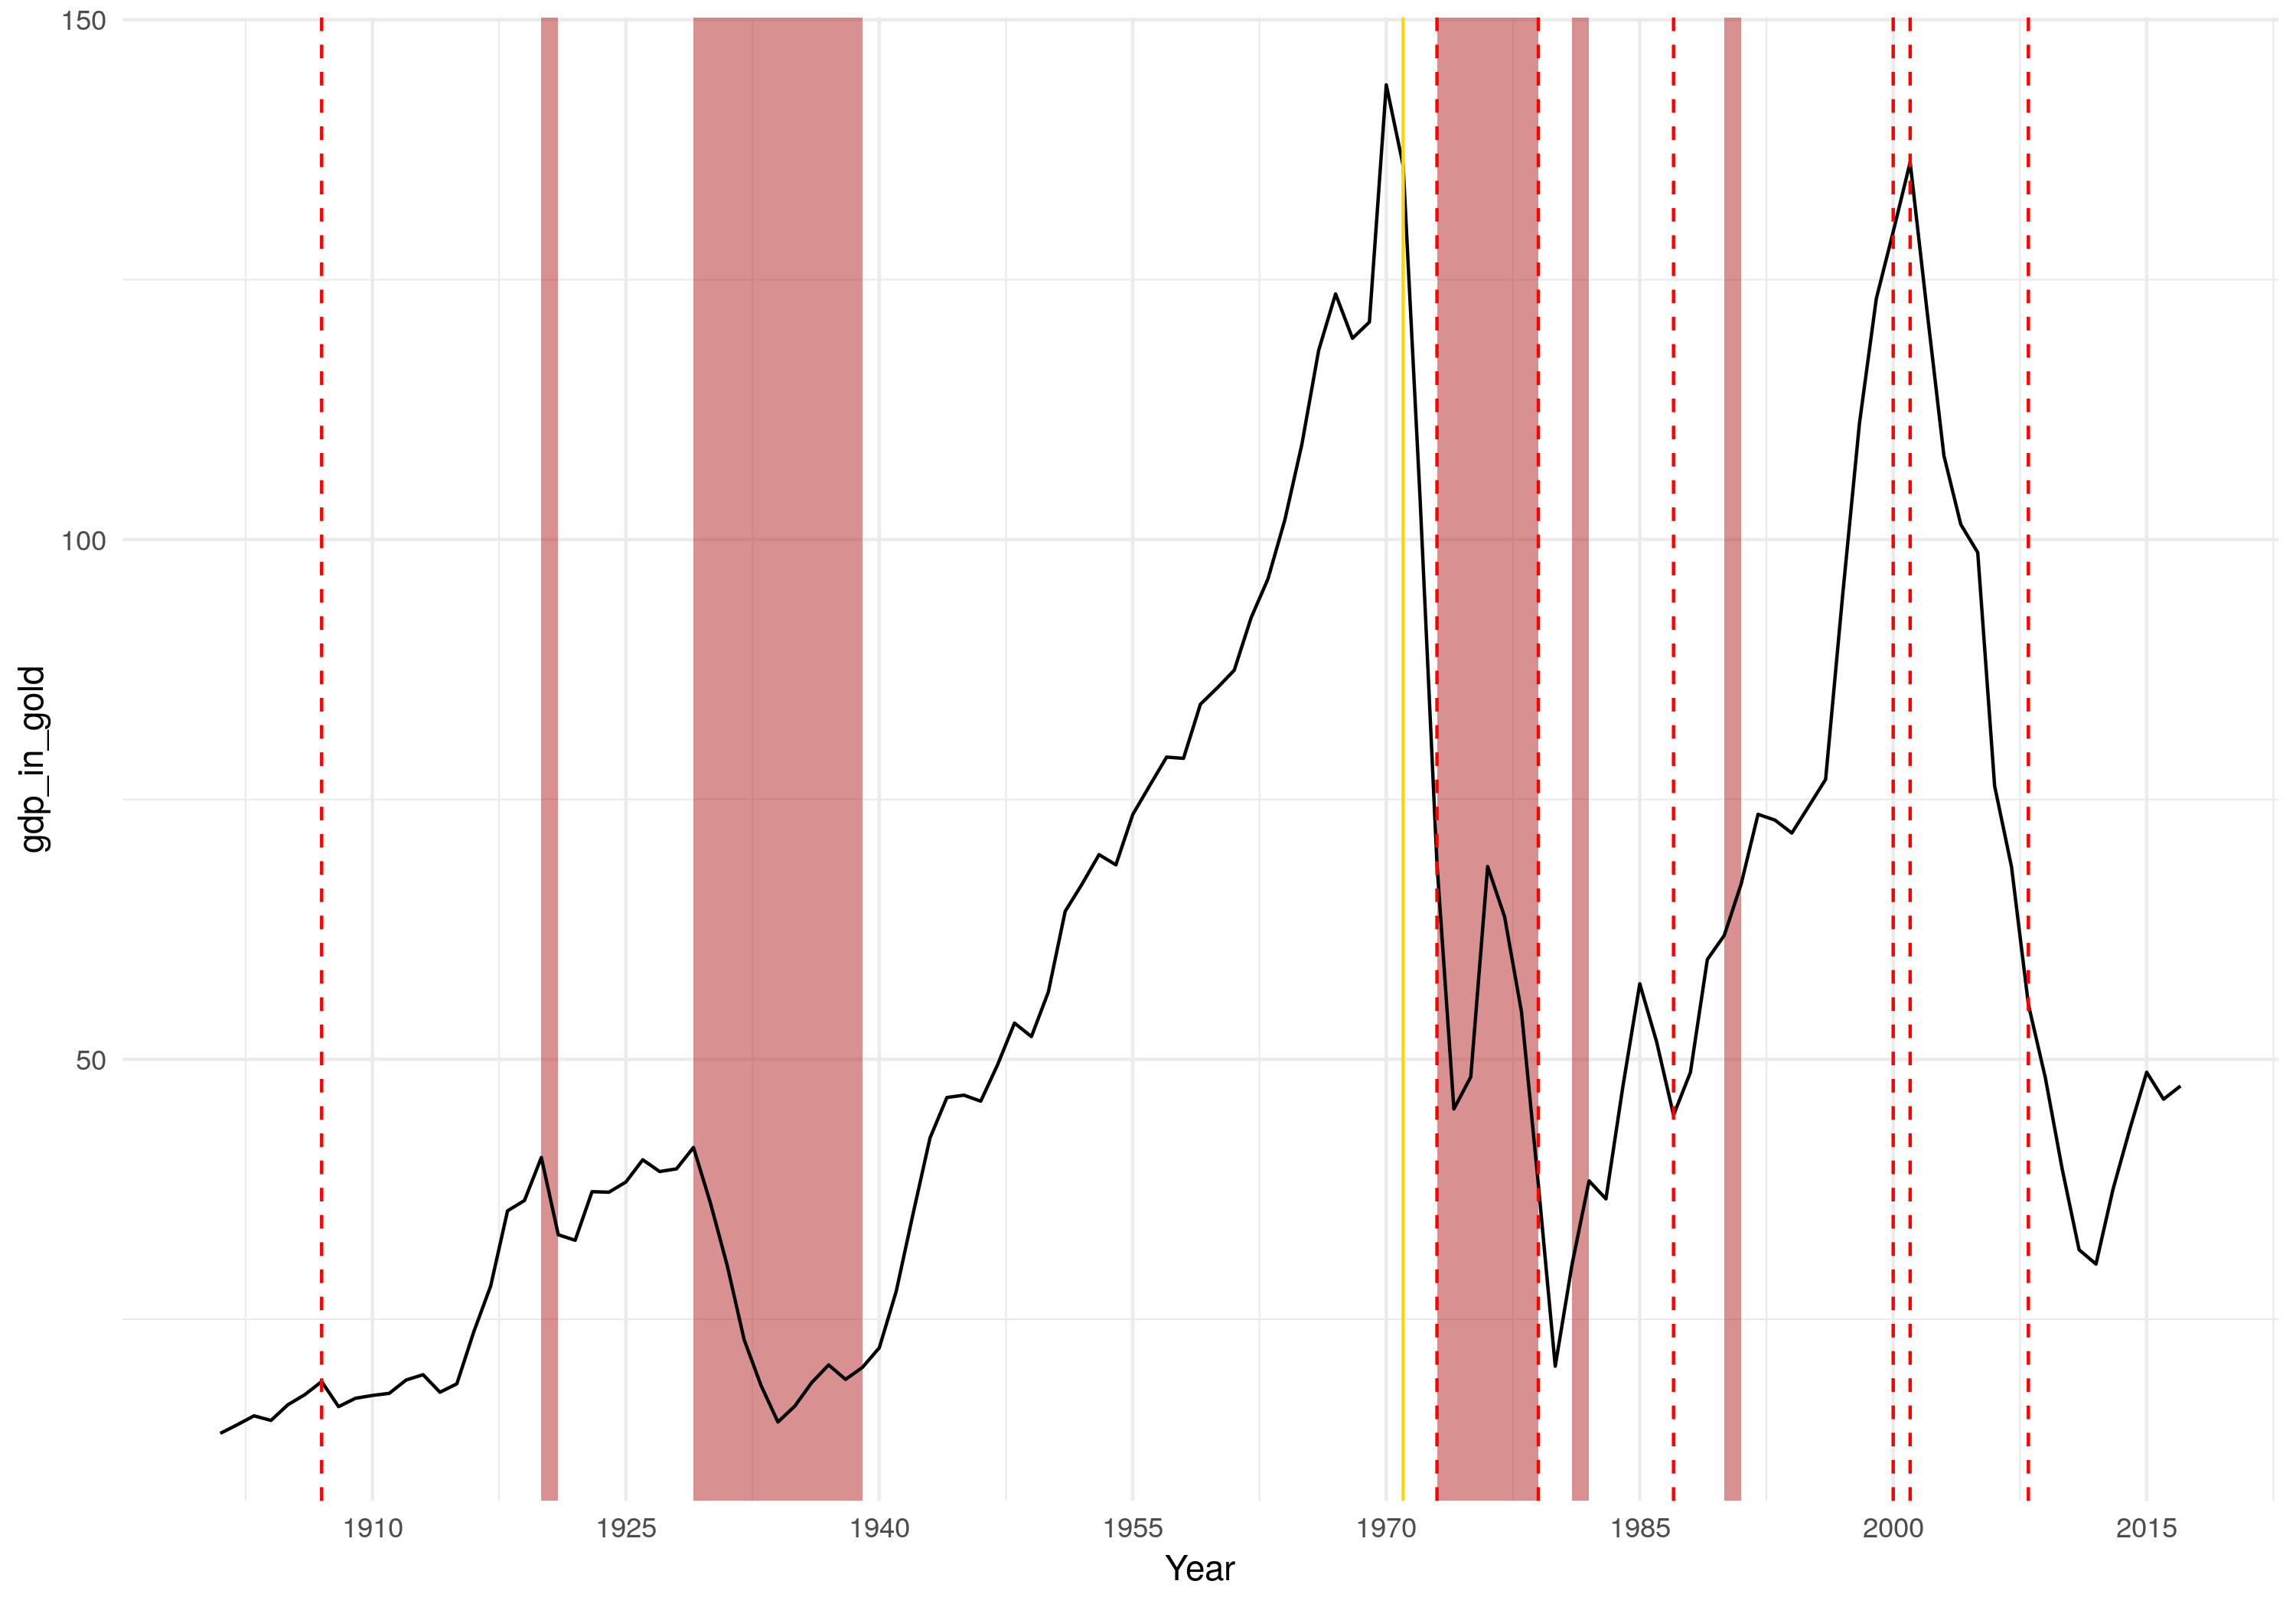
\includegraphics[width=0.75\linewidth]{gdp_in_gold_eda.PNG}}
	\subfigure[Salario expresado en Oro]{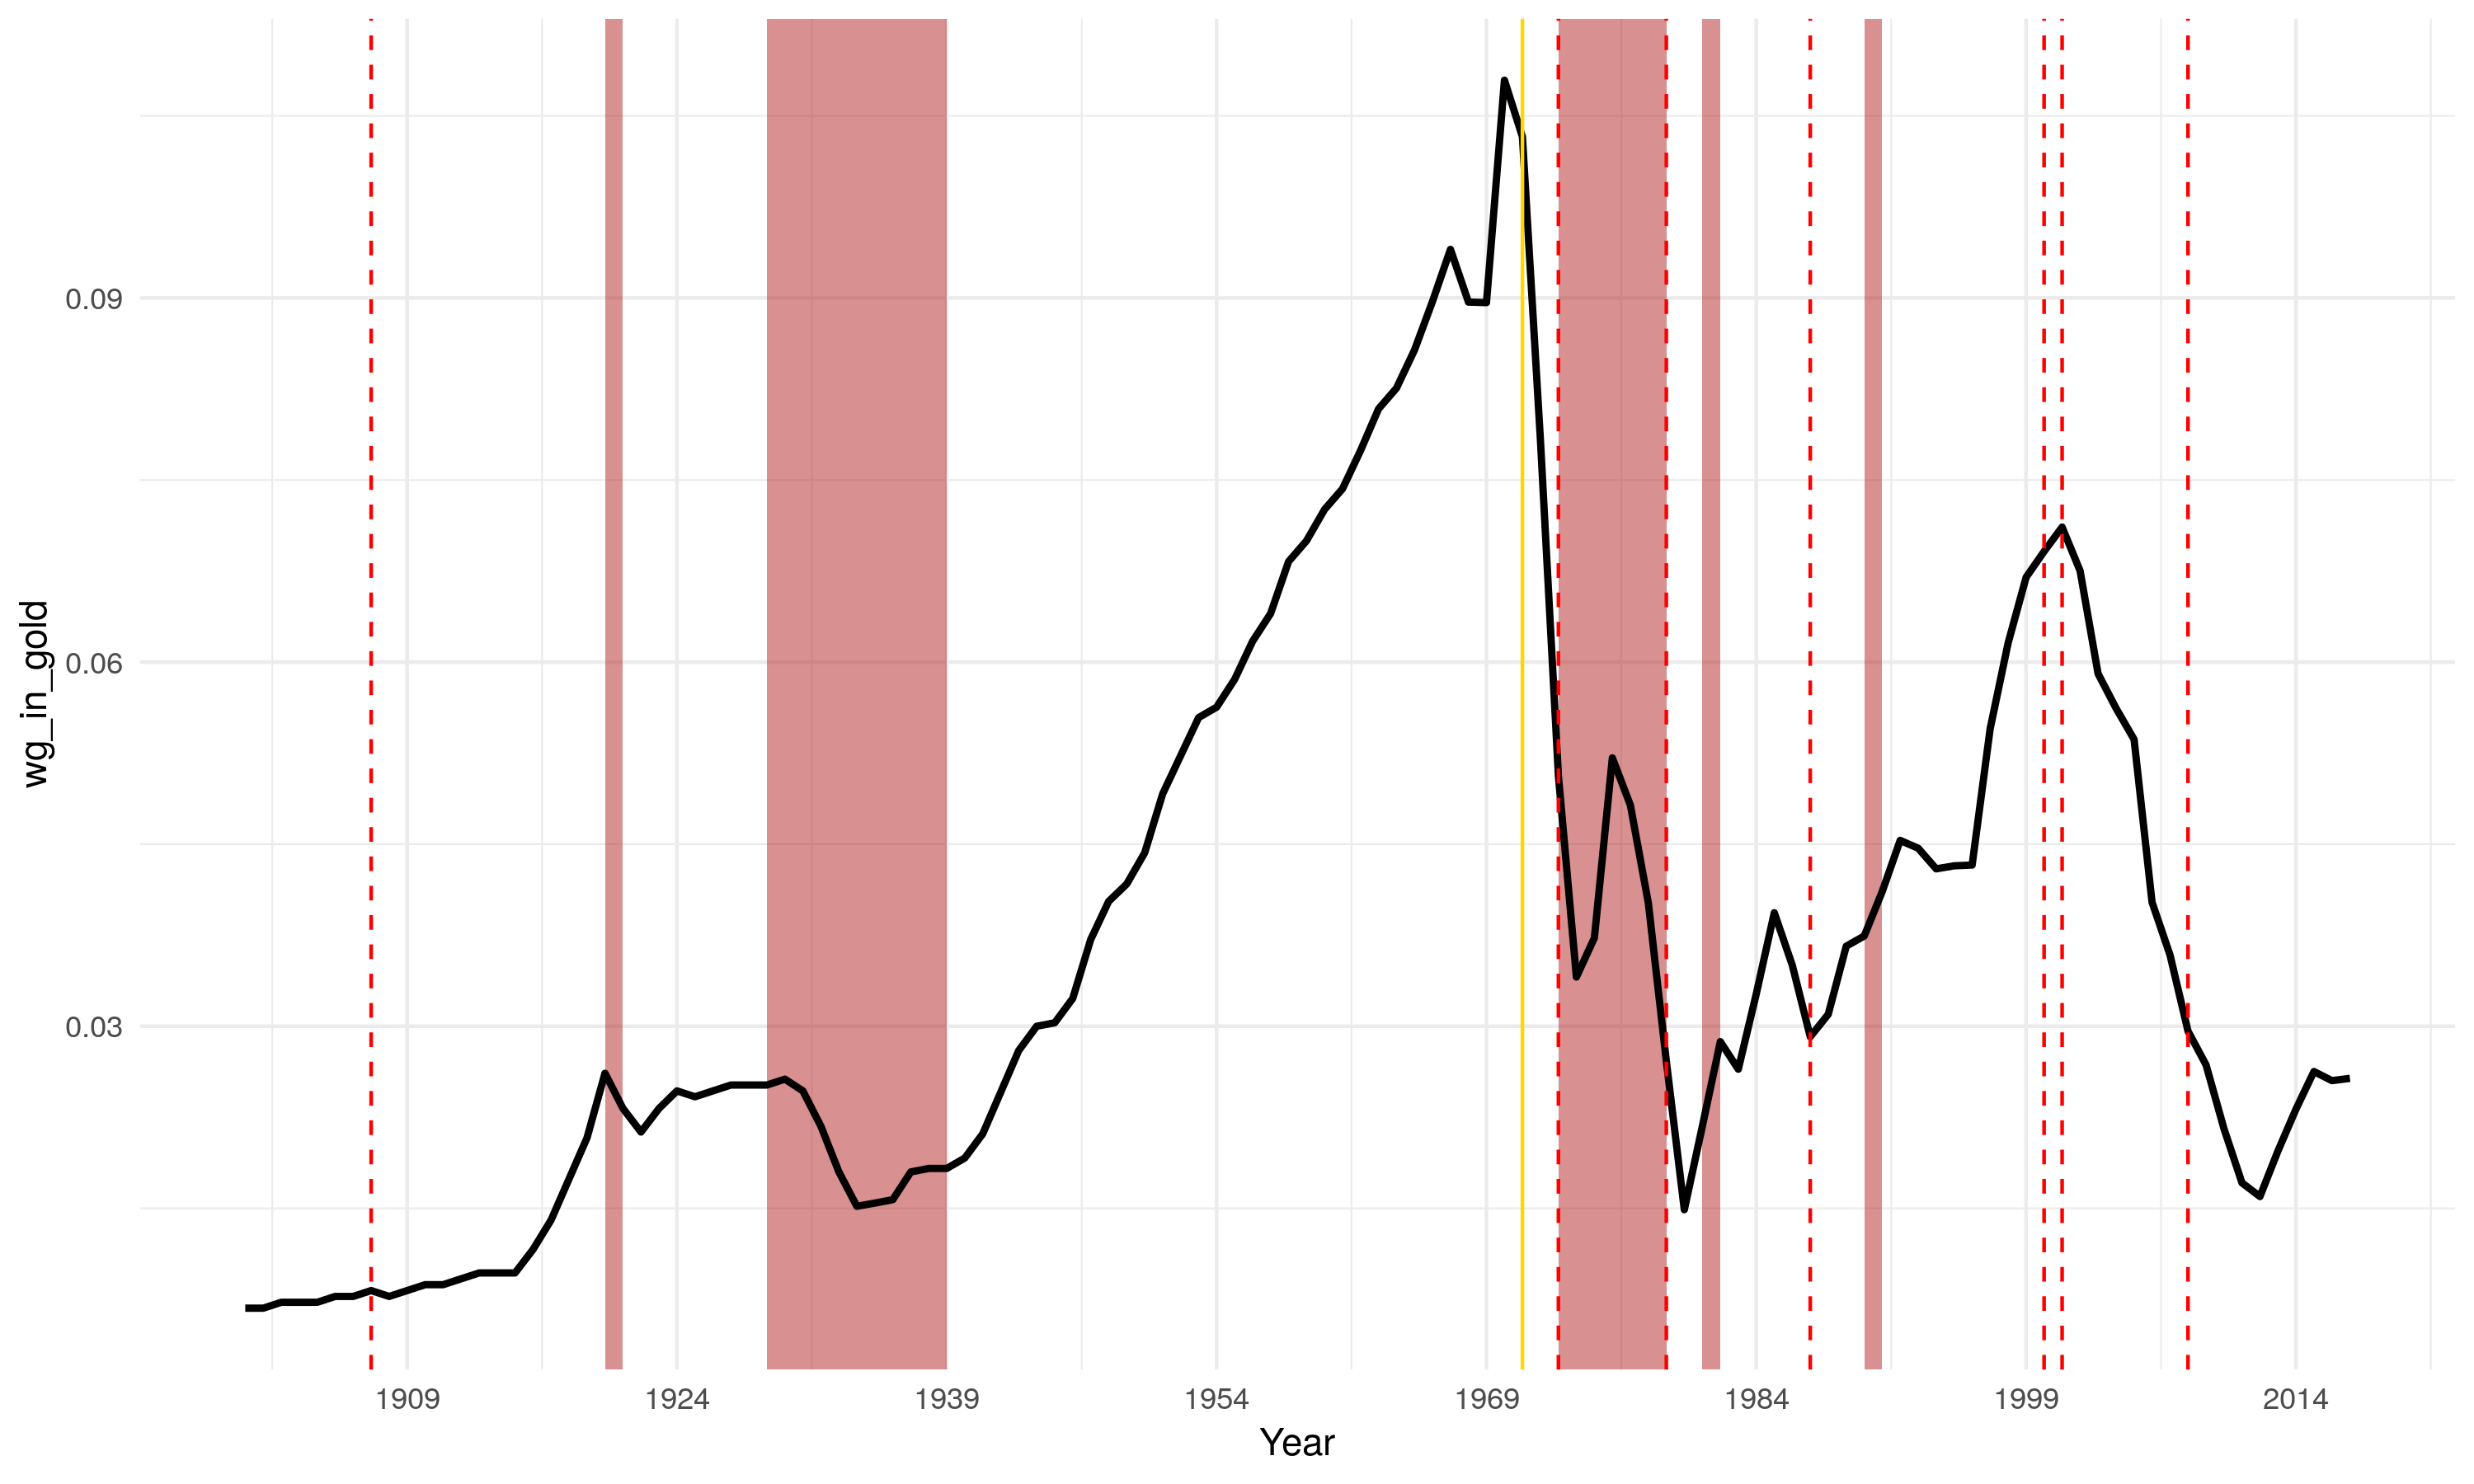
\includegraphics[width=0.75\linewidth]{wg_in_gold_eda.PNG}}
	\caption{Series Expresadas en Oro. Destacado de crisis conocidas} \label{fig:series_crisis}
\end{figure}


\section{Autocorrelación}

\begin{figure}[H]
	\centering
	\subfigure[PBI expresado en Oro]{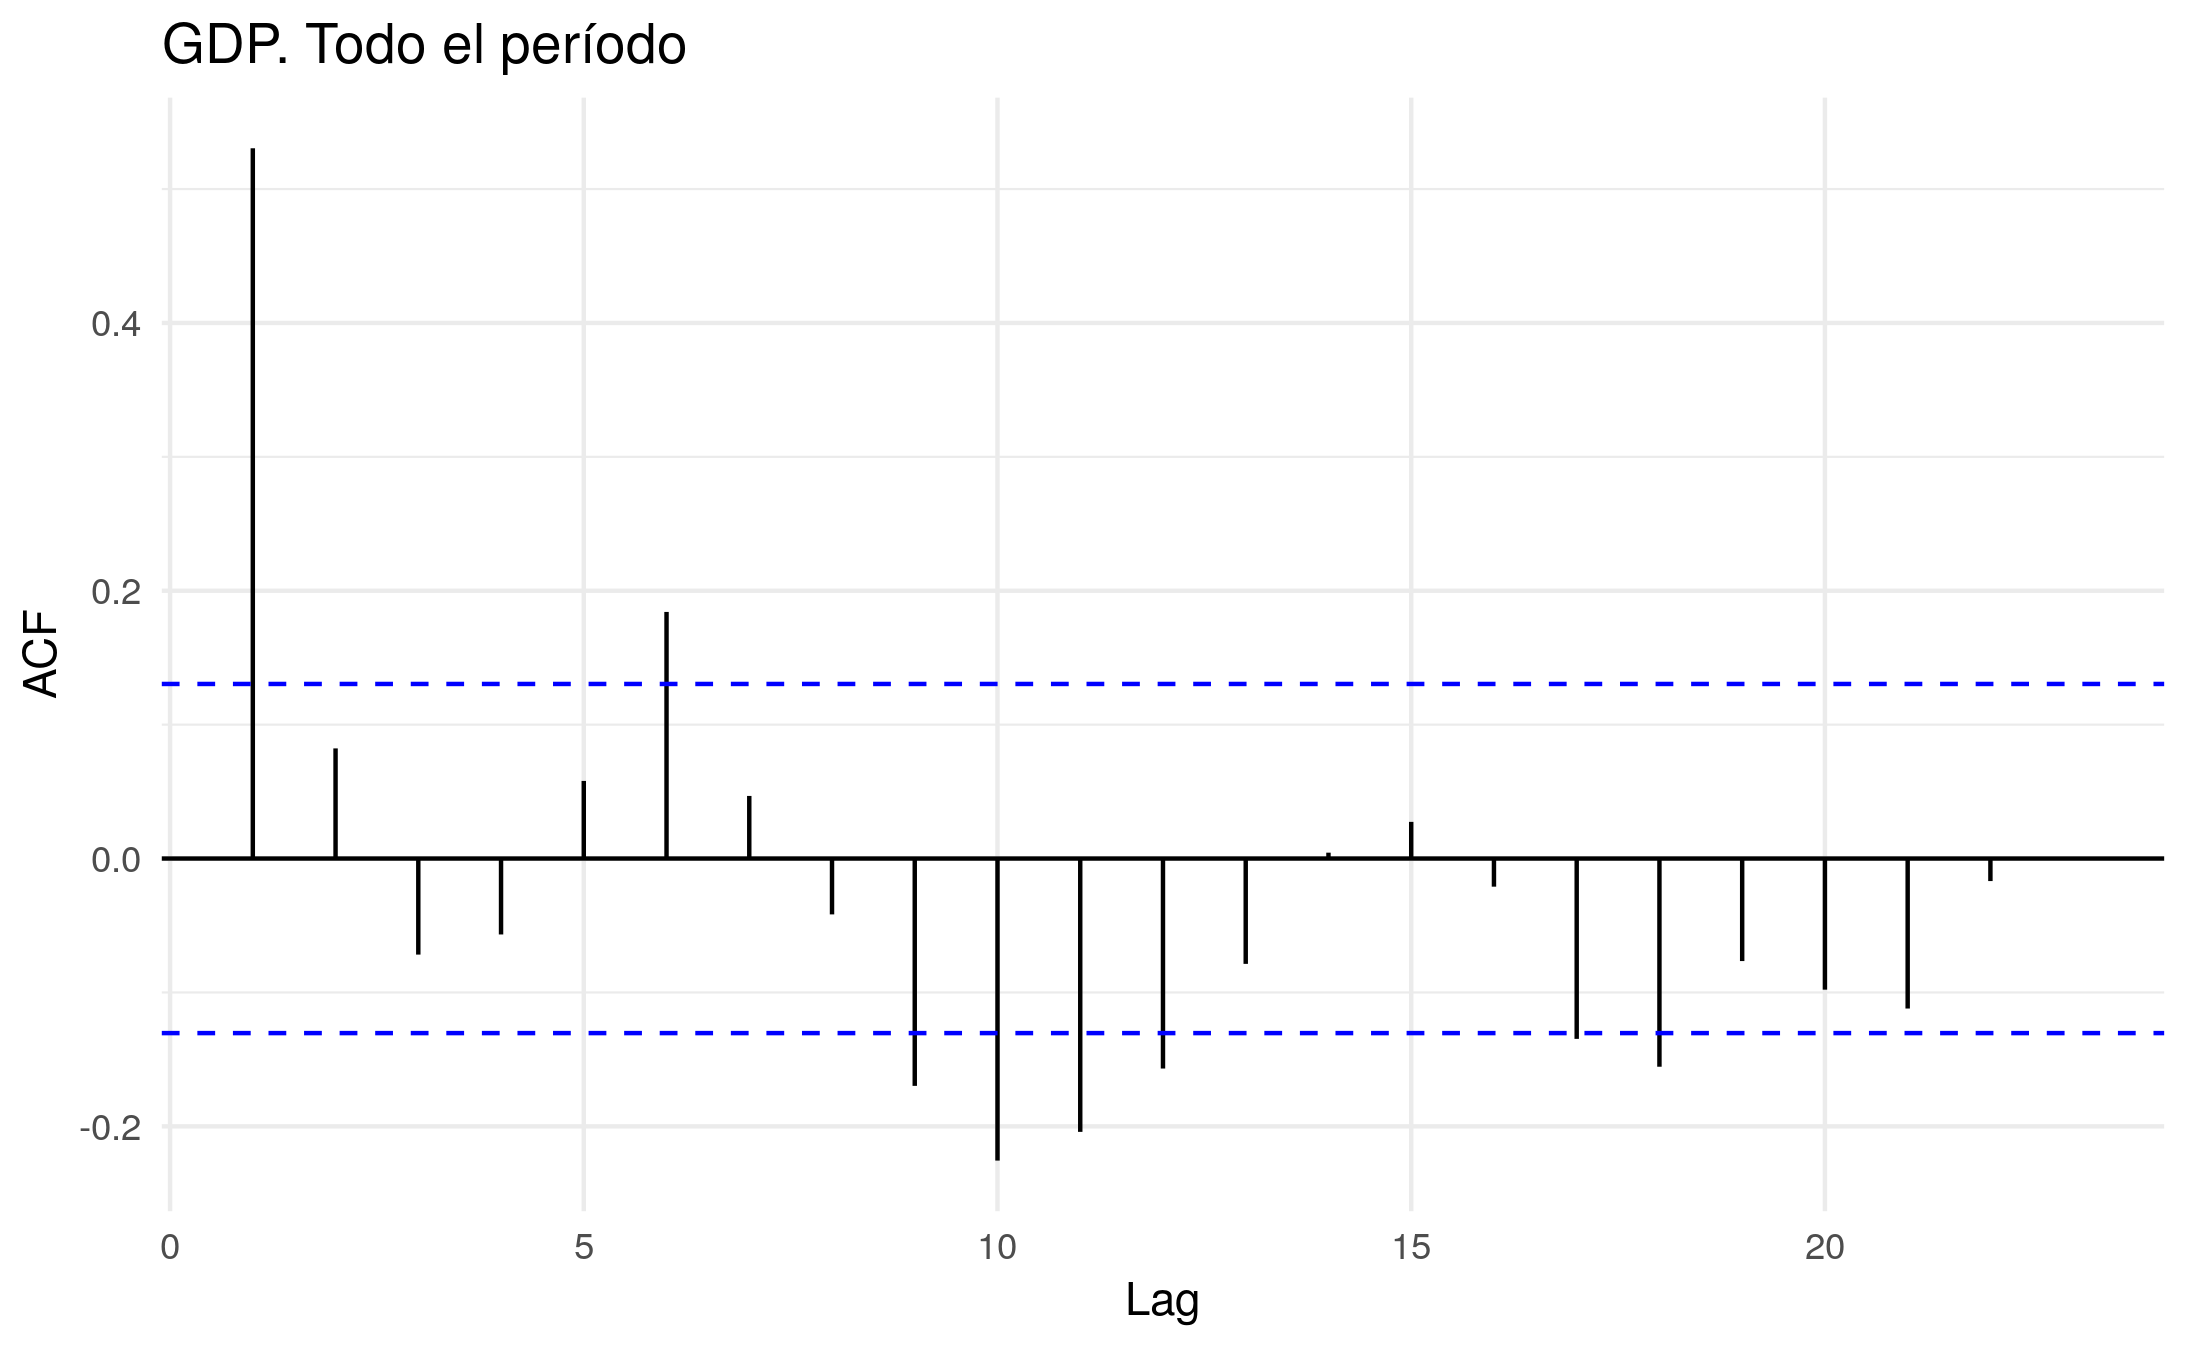
\includegraphics[width=0.75\linewidth]{Autocorrelacion_gdp.png}}
	\subfigure[Salario expresado en Oro]{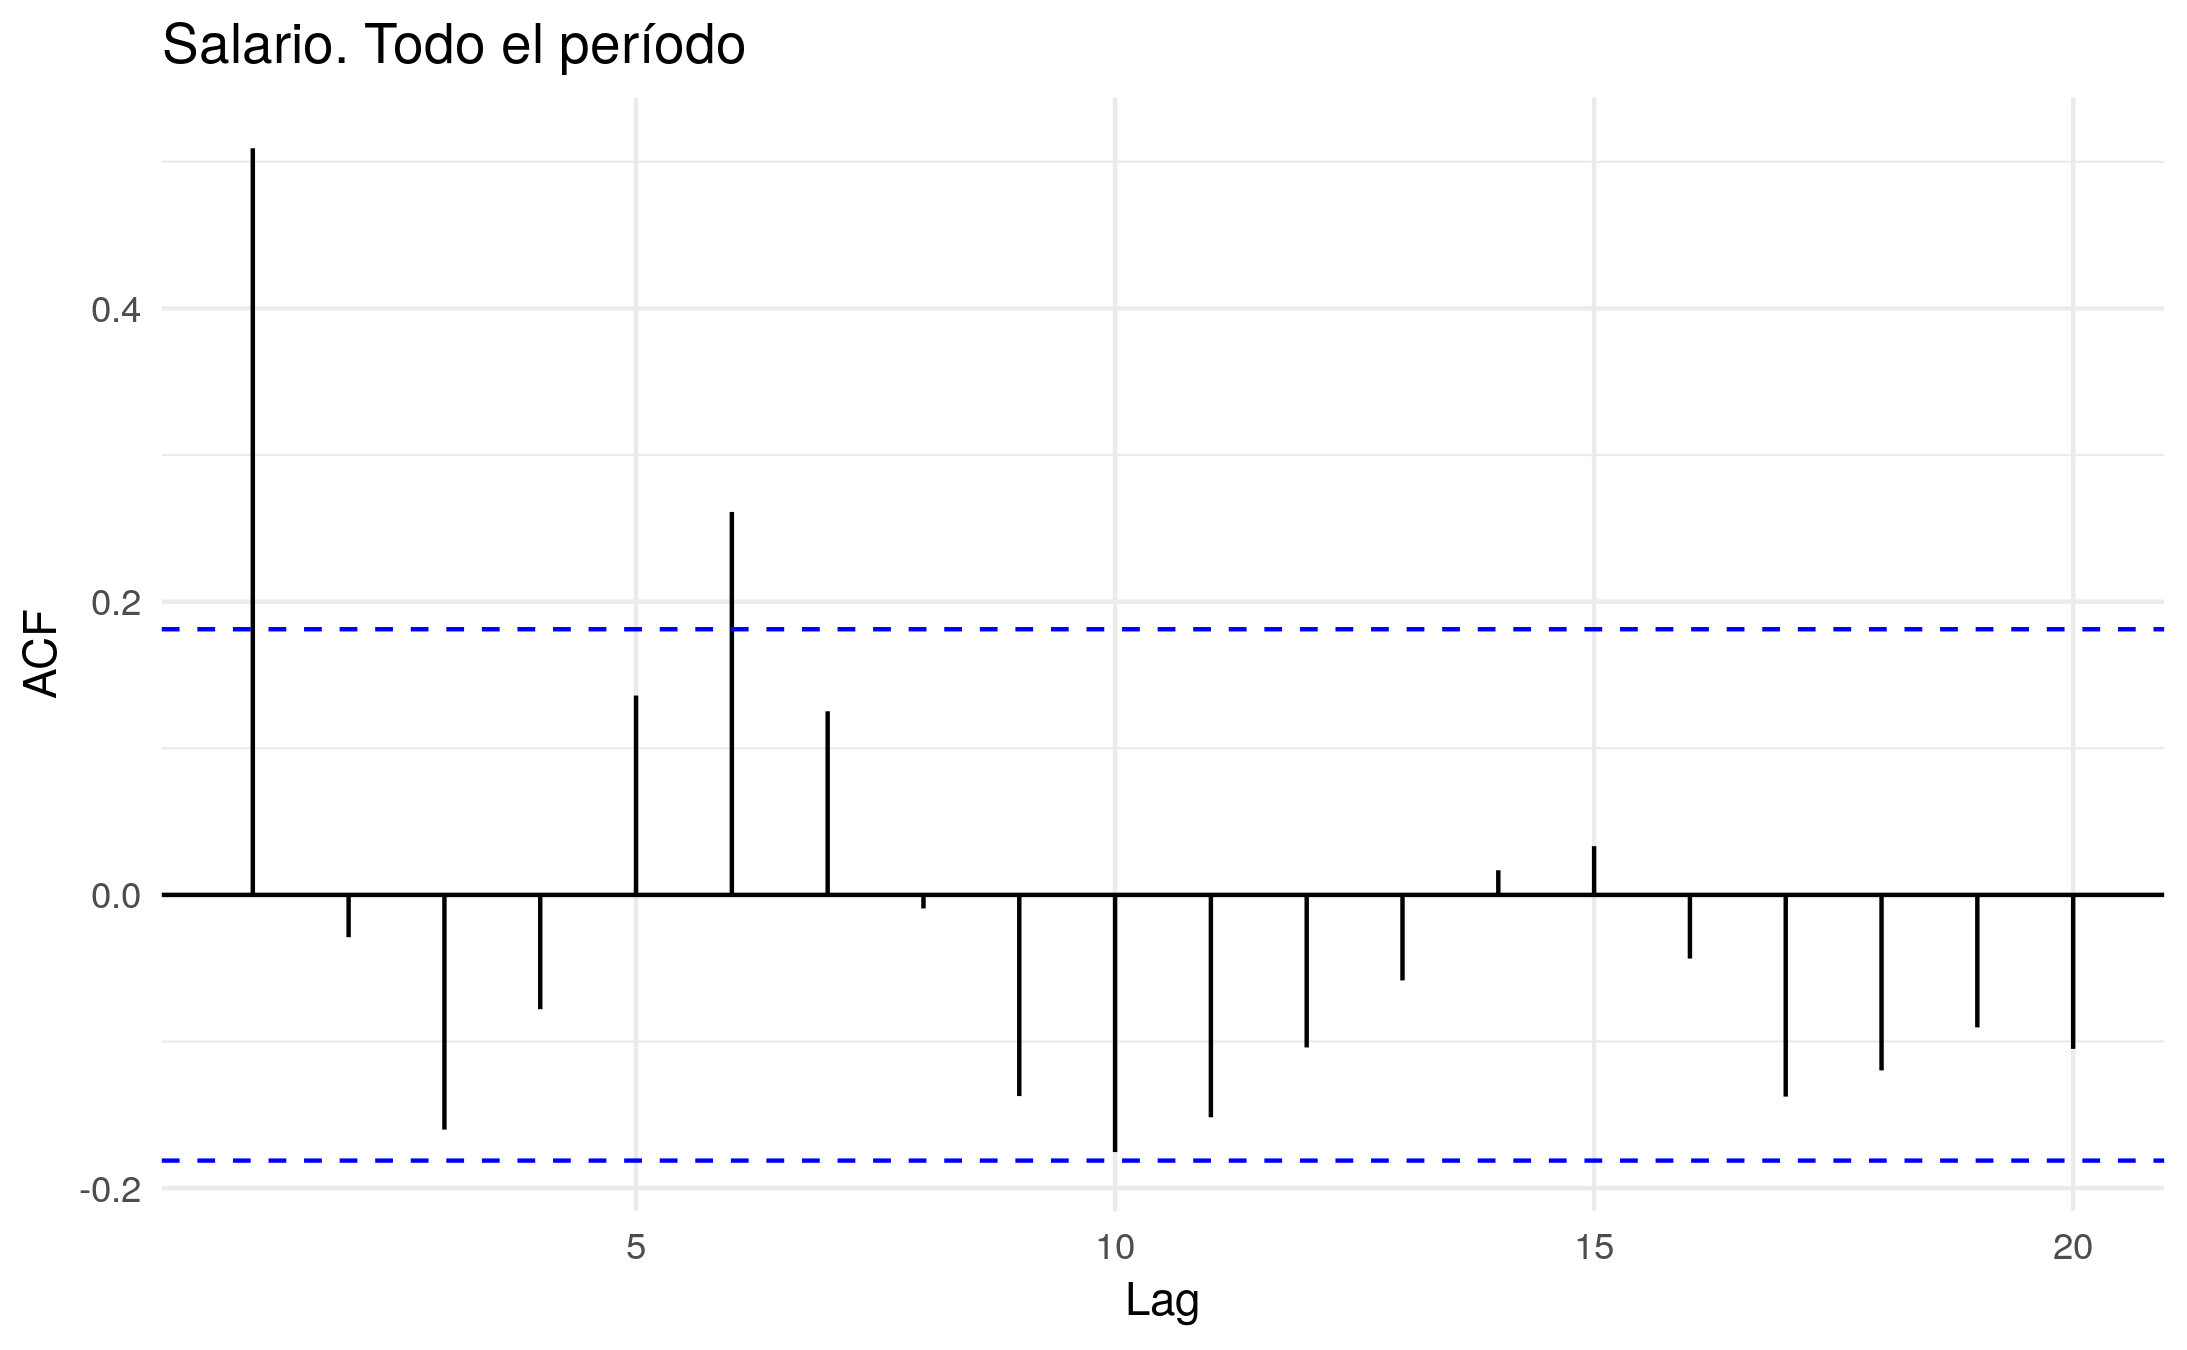
\includegraphics[width=0.75\linewidth]{Autocorrelacion_wg.png}}
	\caption{Autocorrelación de las series} \label{fig:autocorrelacion_tot}
\end{figure}


\begin{figure}[H]
	\centering
	\subfigure[PBI antes 1971]{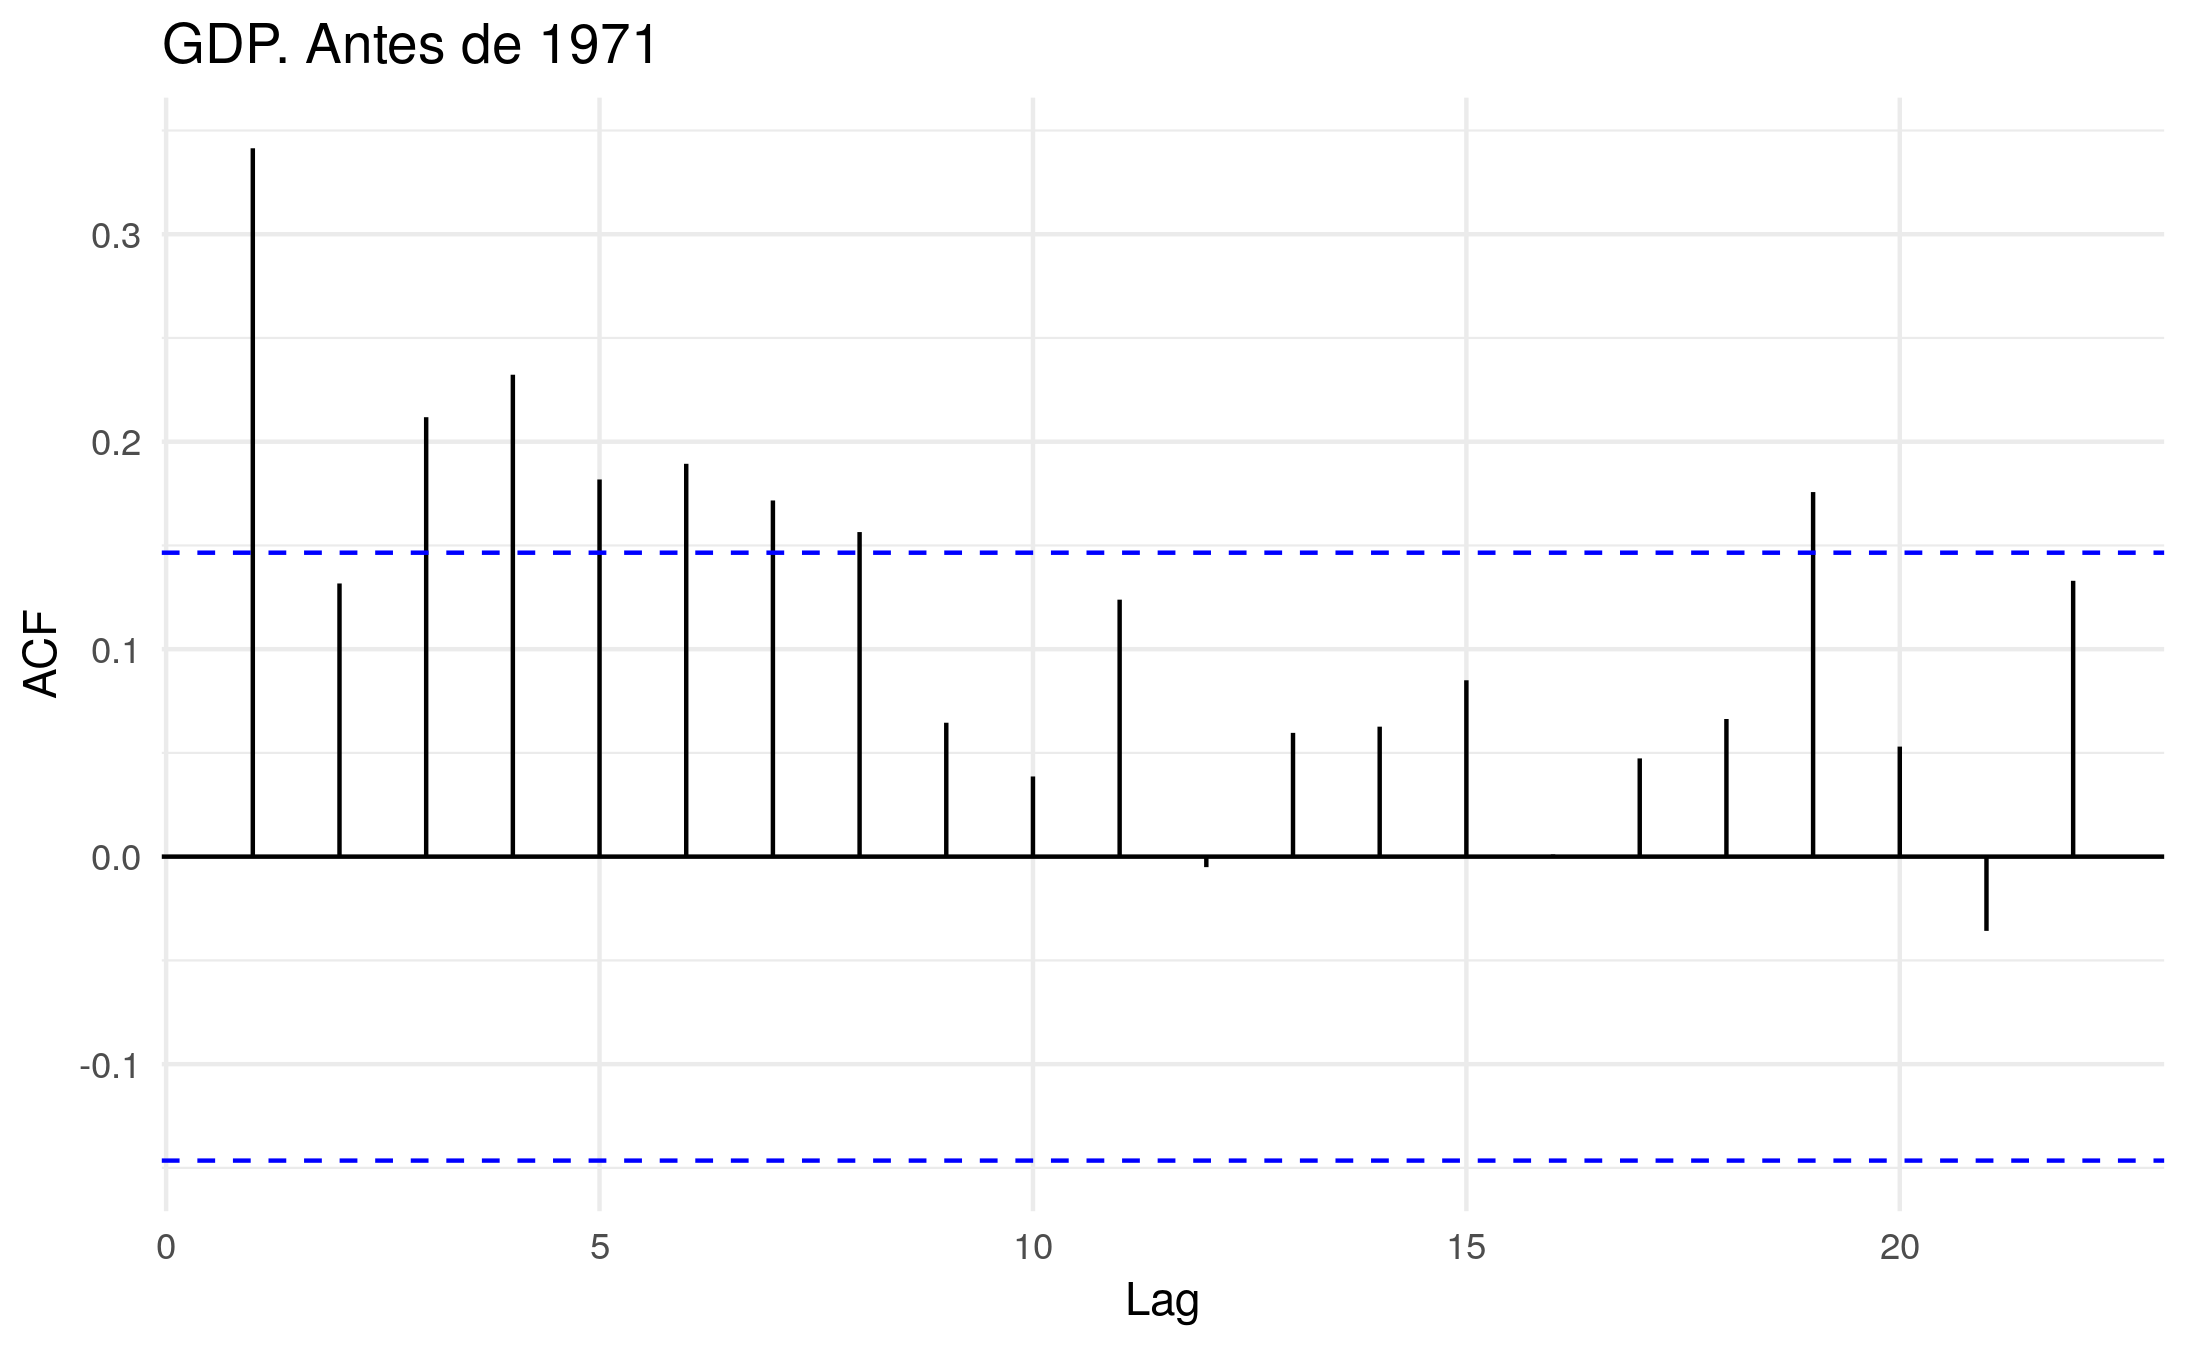
\includegraphics[width=0.49\linewidth]{Autocorrelacion_gdp_pre71.png}}
	\subfigure[PBI después 1971]{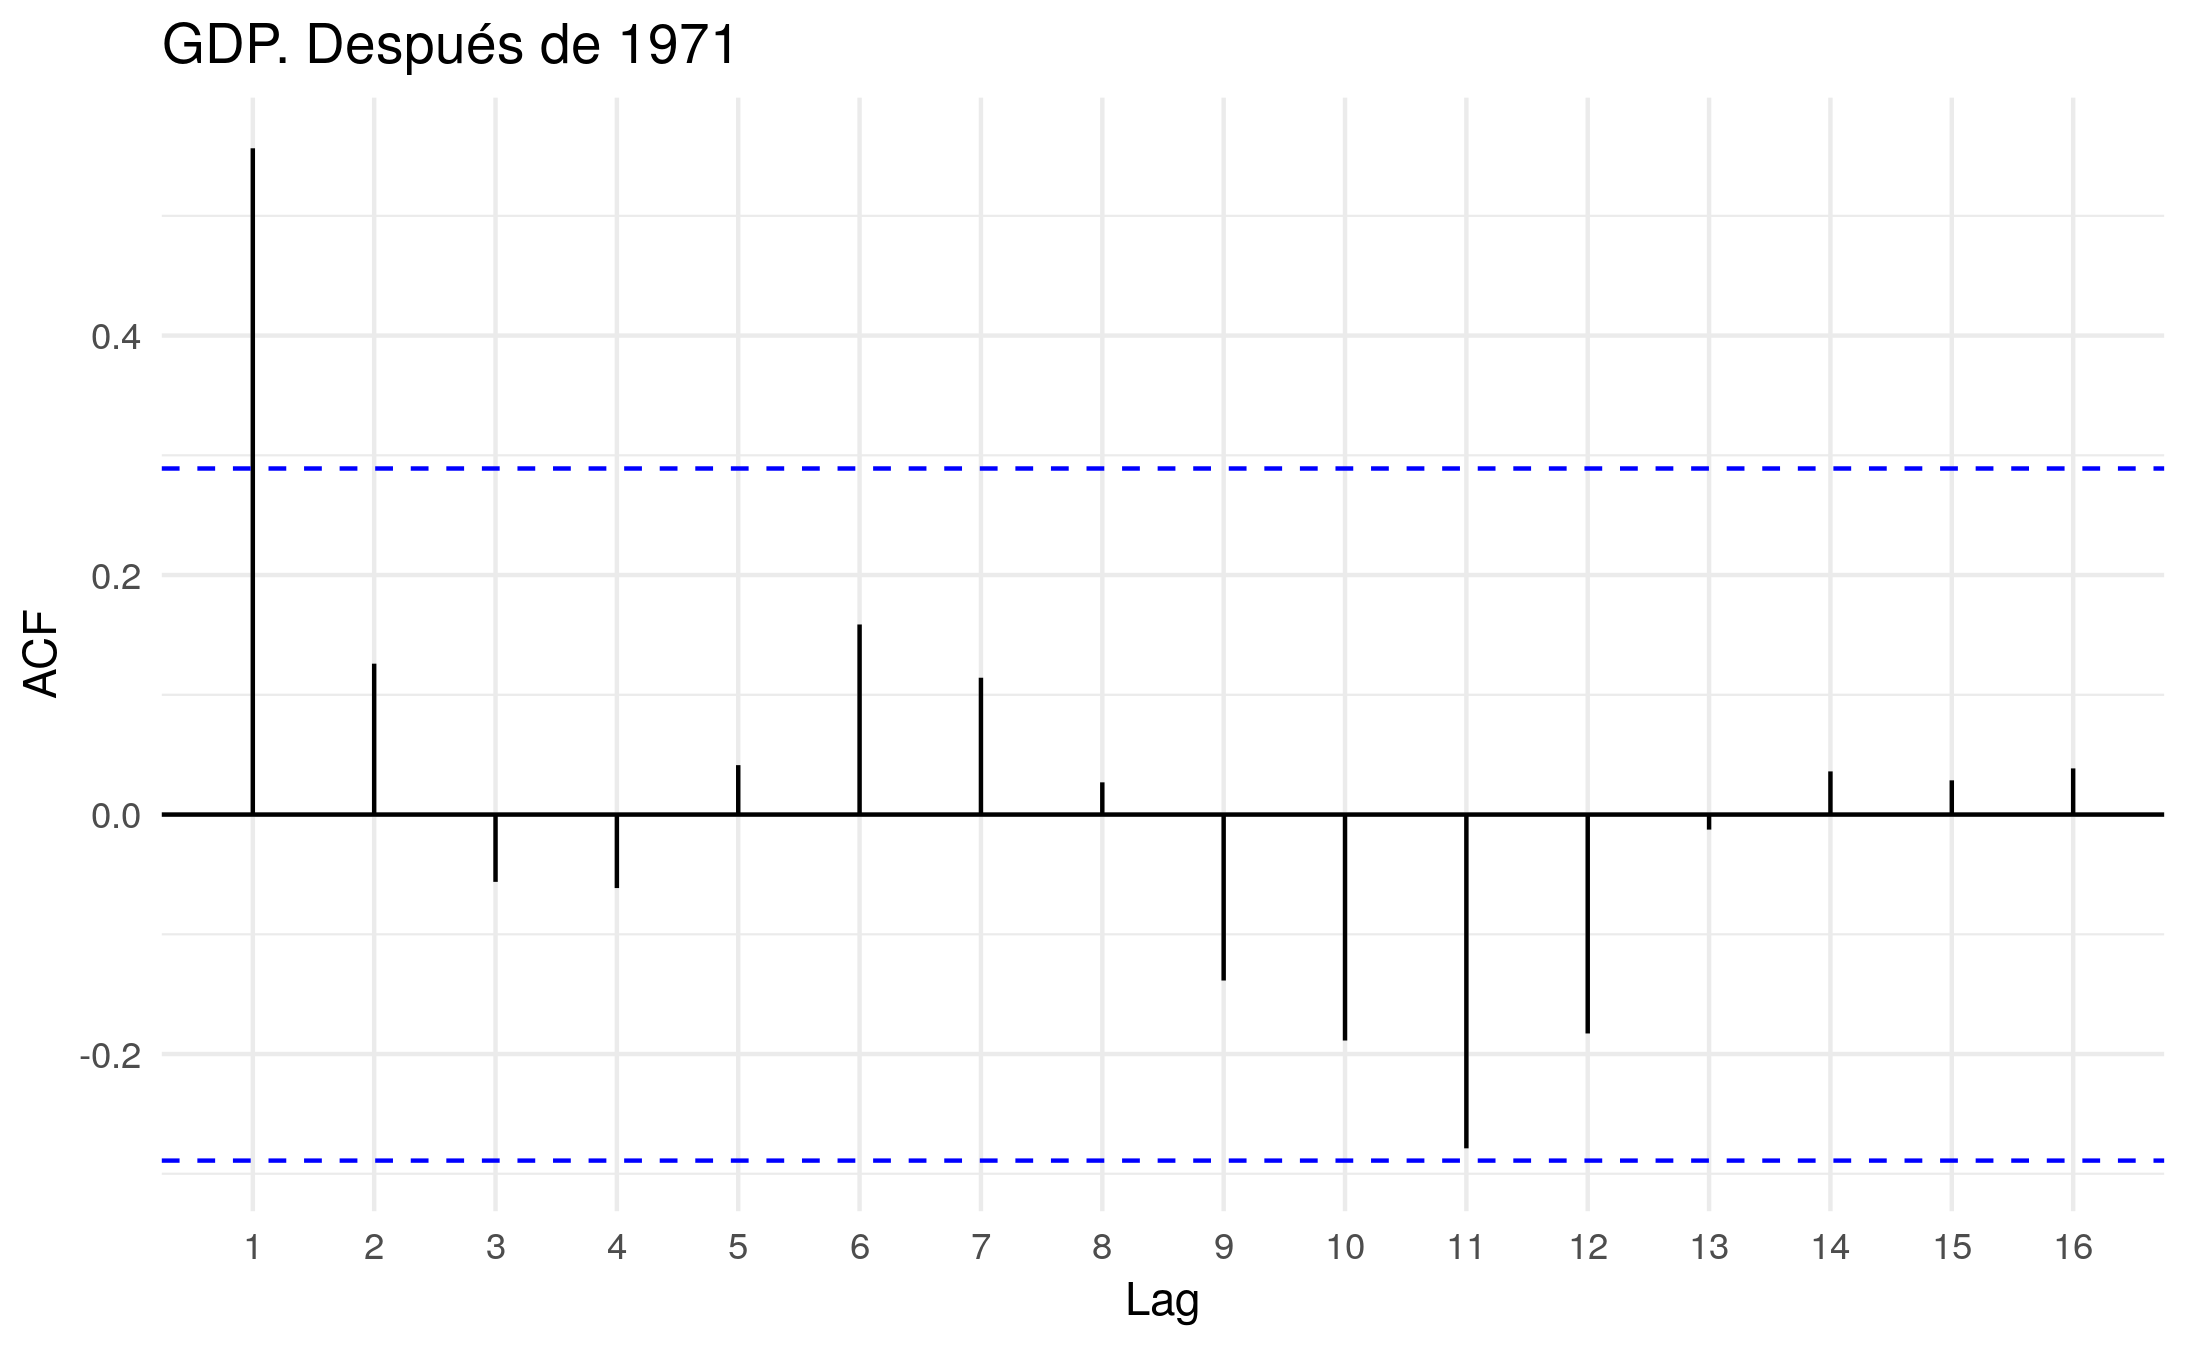
\includegraphics[width=0.49\linewidth]{Autocorrelacion_gdp_post71.png}}
	\subfigure[Salario antes 1971]{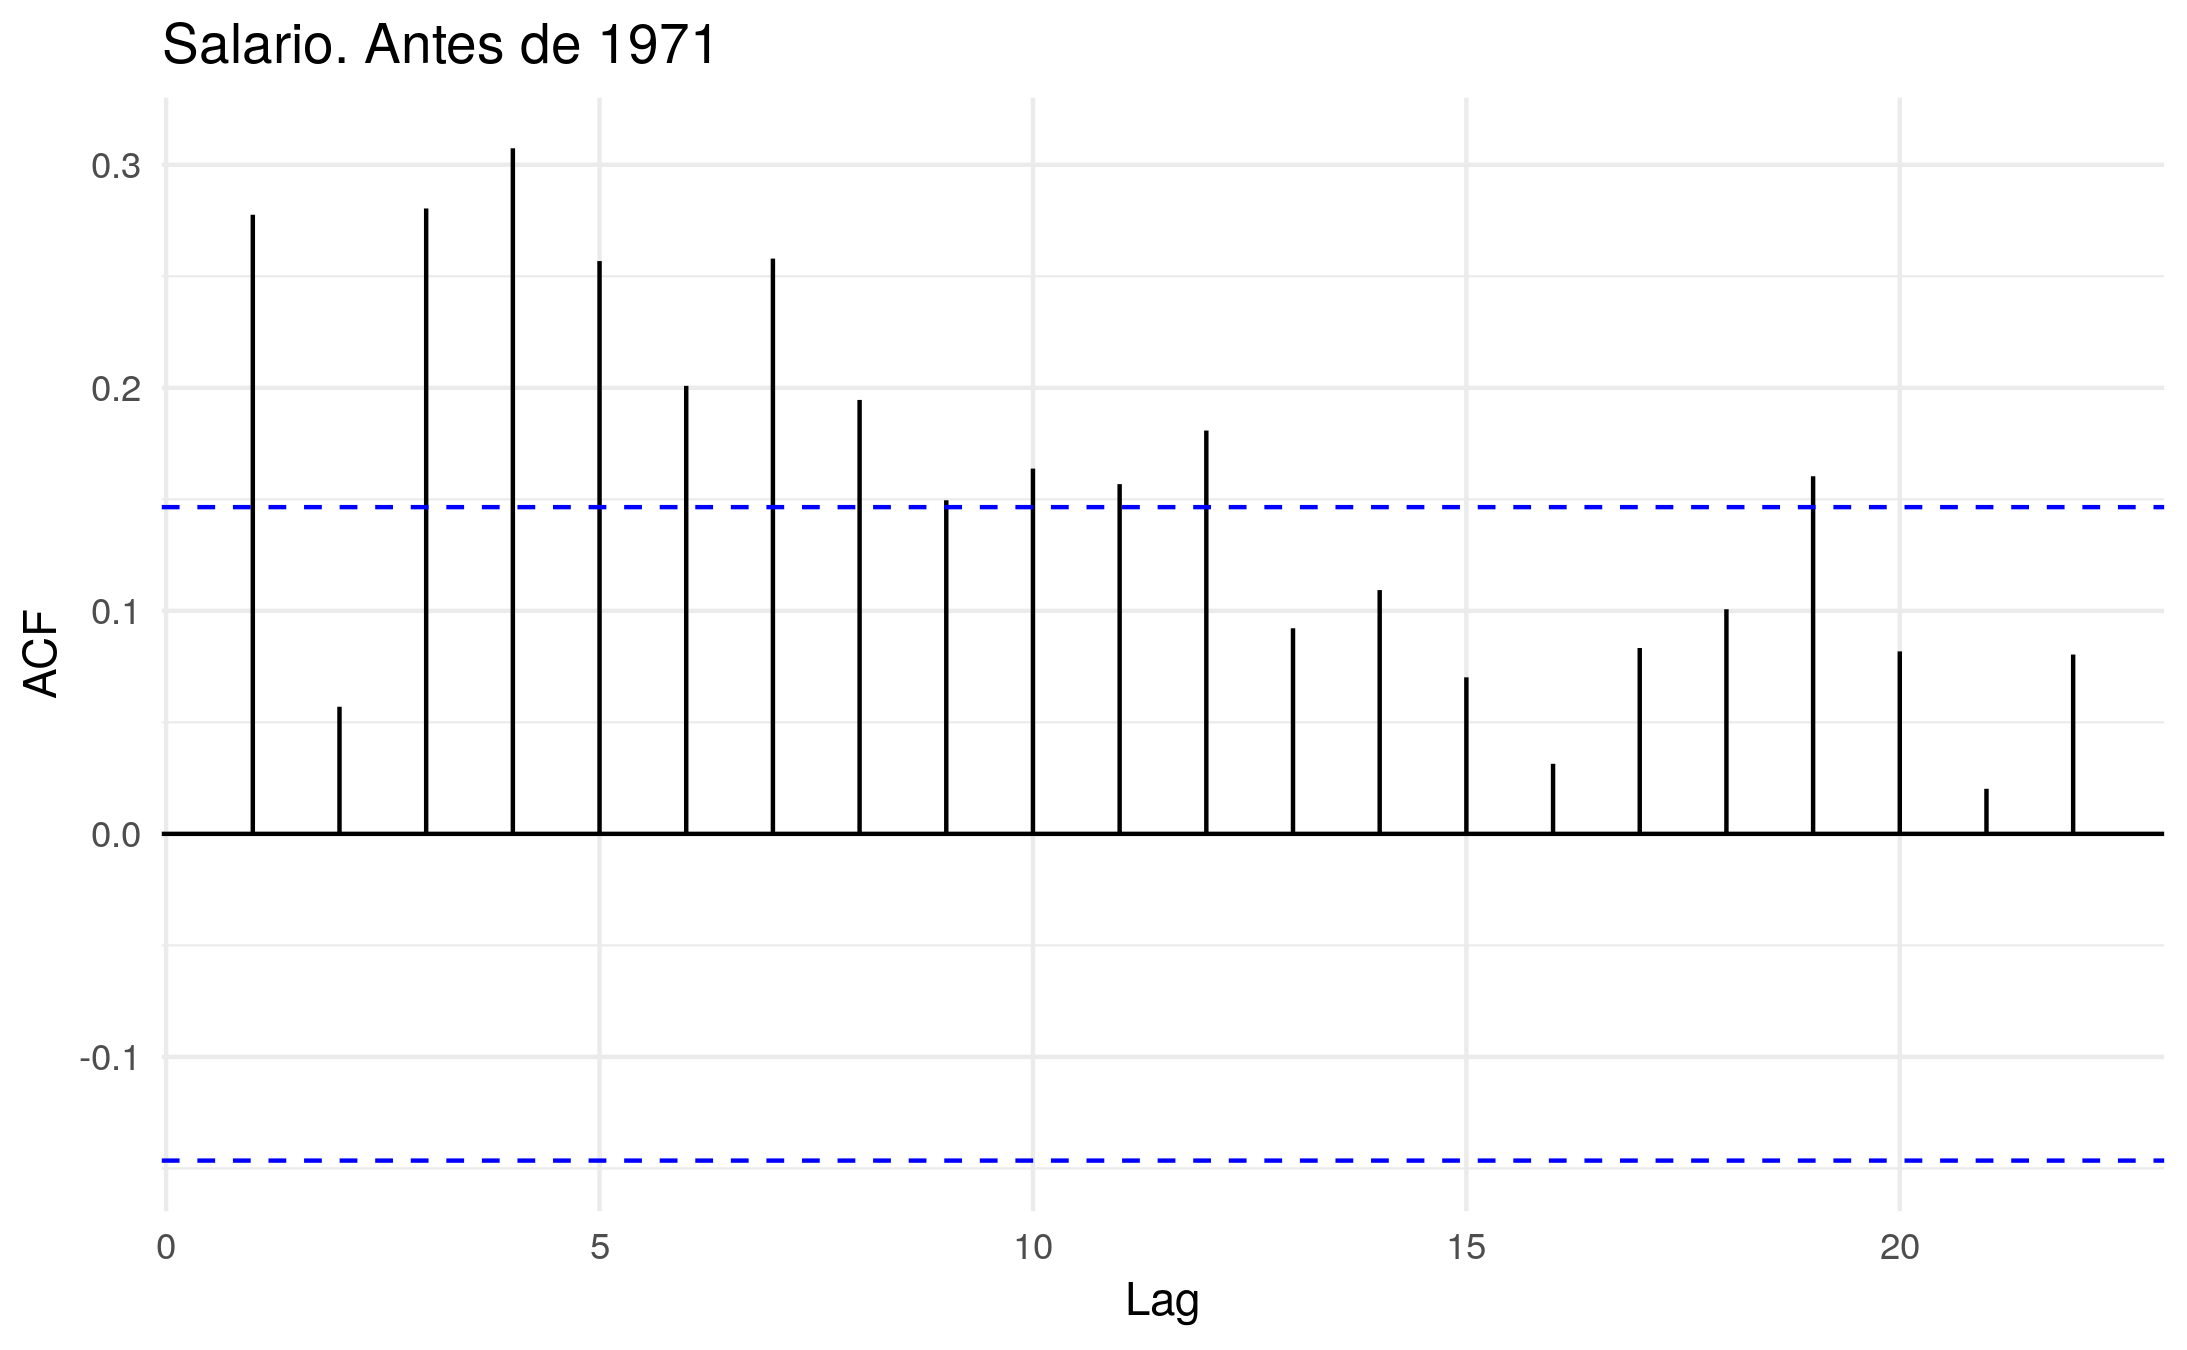
\includegraphics[width=0.49\linewidth]{Autocorrelacion_wg_pre71.png}}
	\subfigure[Salario después 1971]{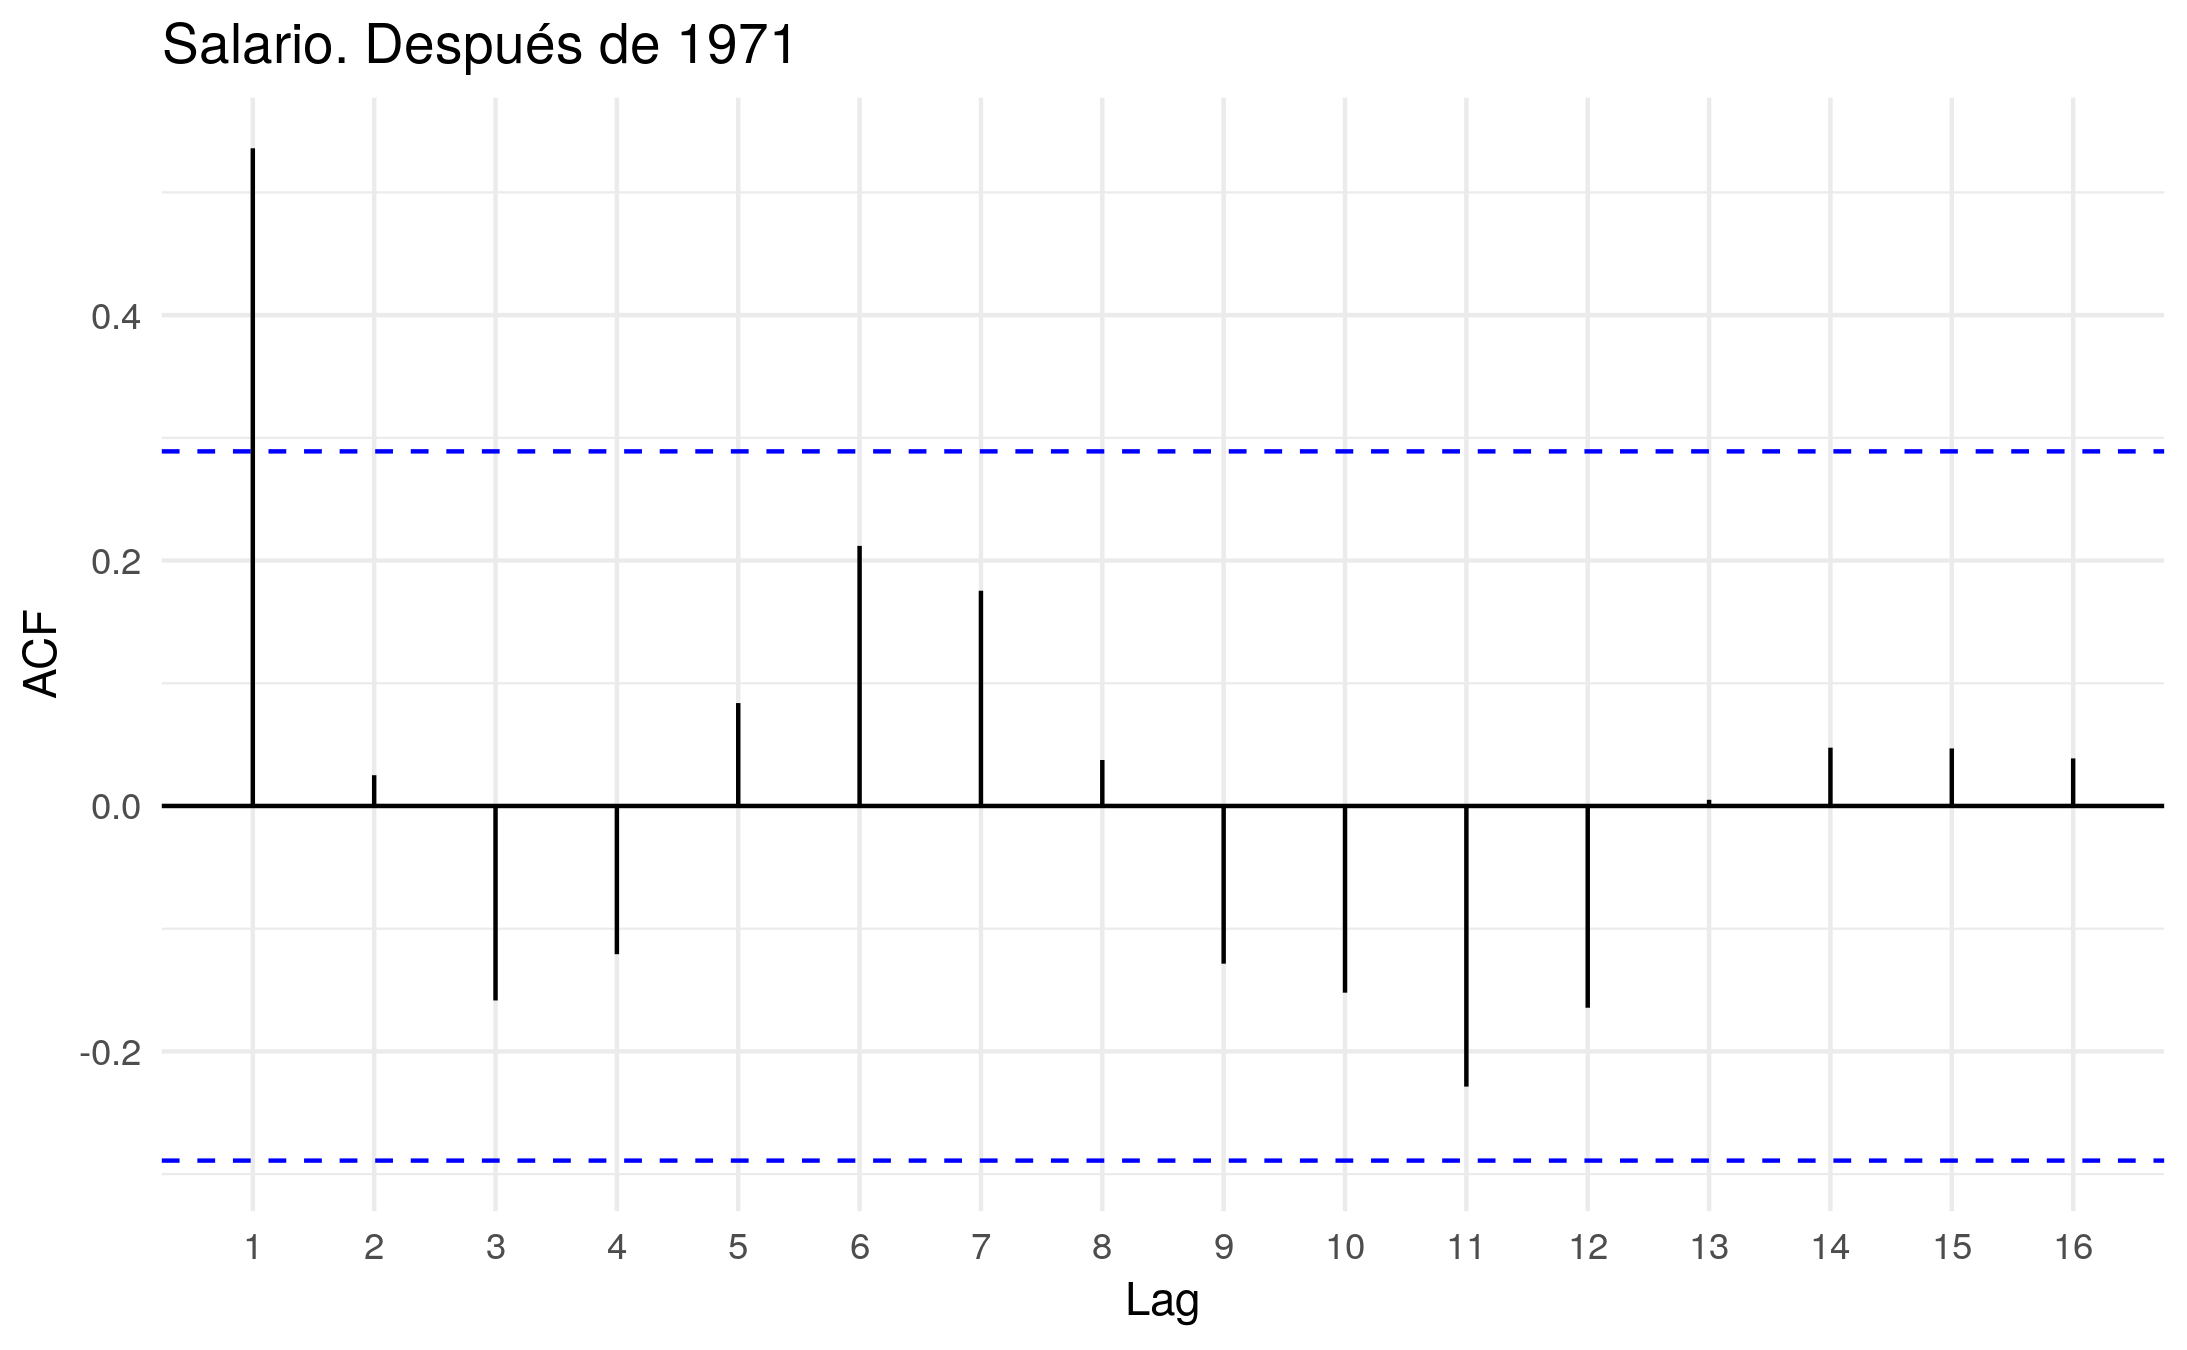
\includegraphics[width=0.49\linewidth]{Autocorrelacion_wg_post71.png}}
	\caption{Autocorrelación de las series} \label{fig:autocorrelacion_grp}
\end{figure}


\section{ARIMA}

\begin{figure}[H]
	\centering
	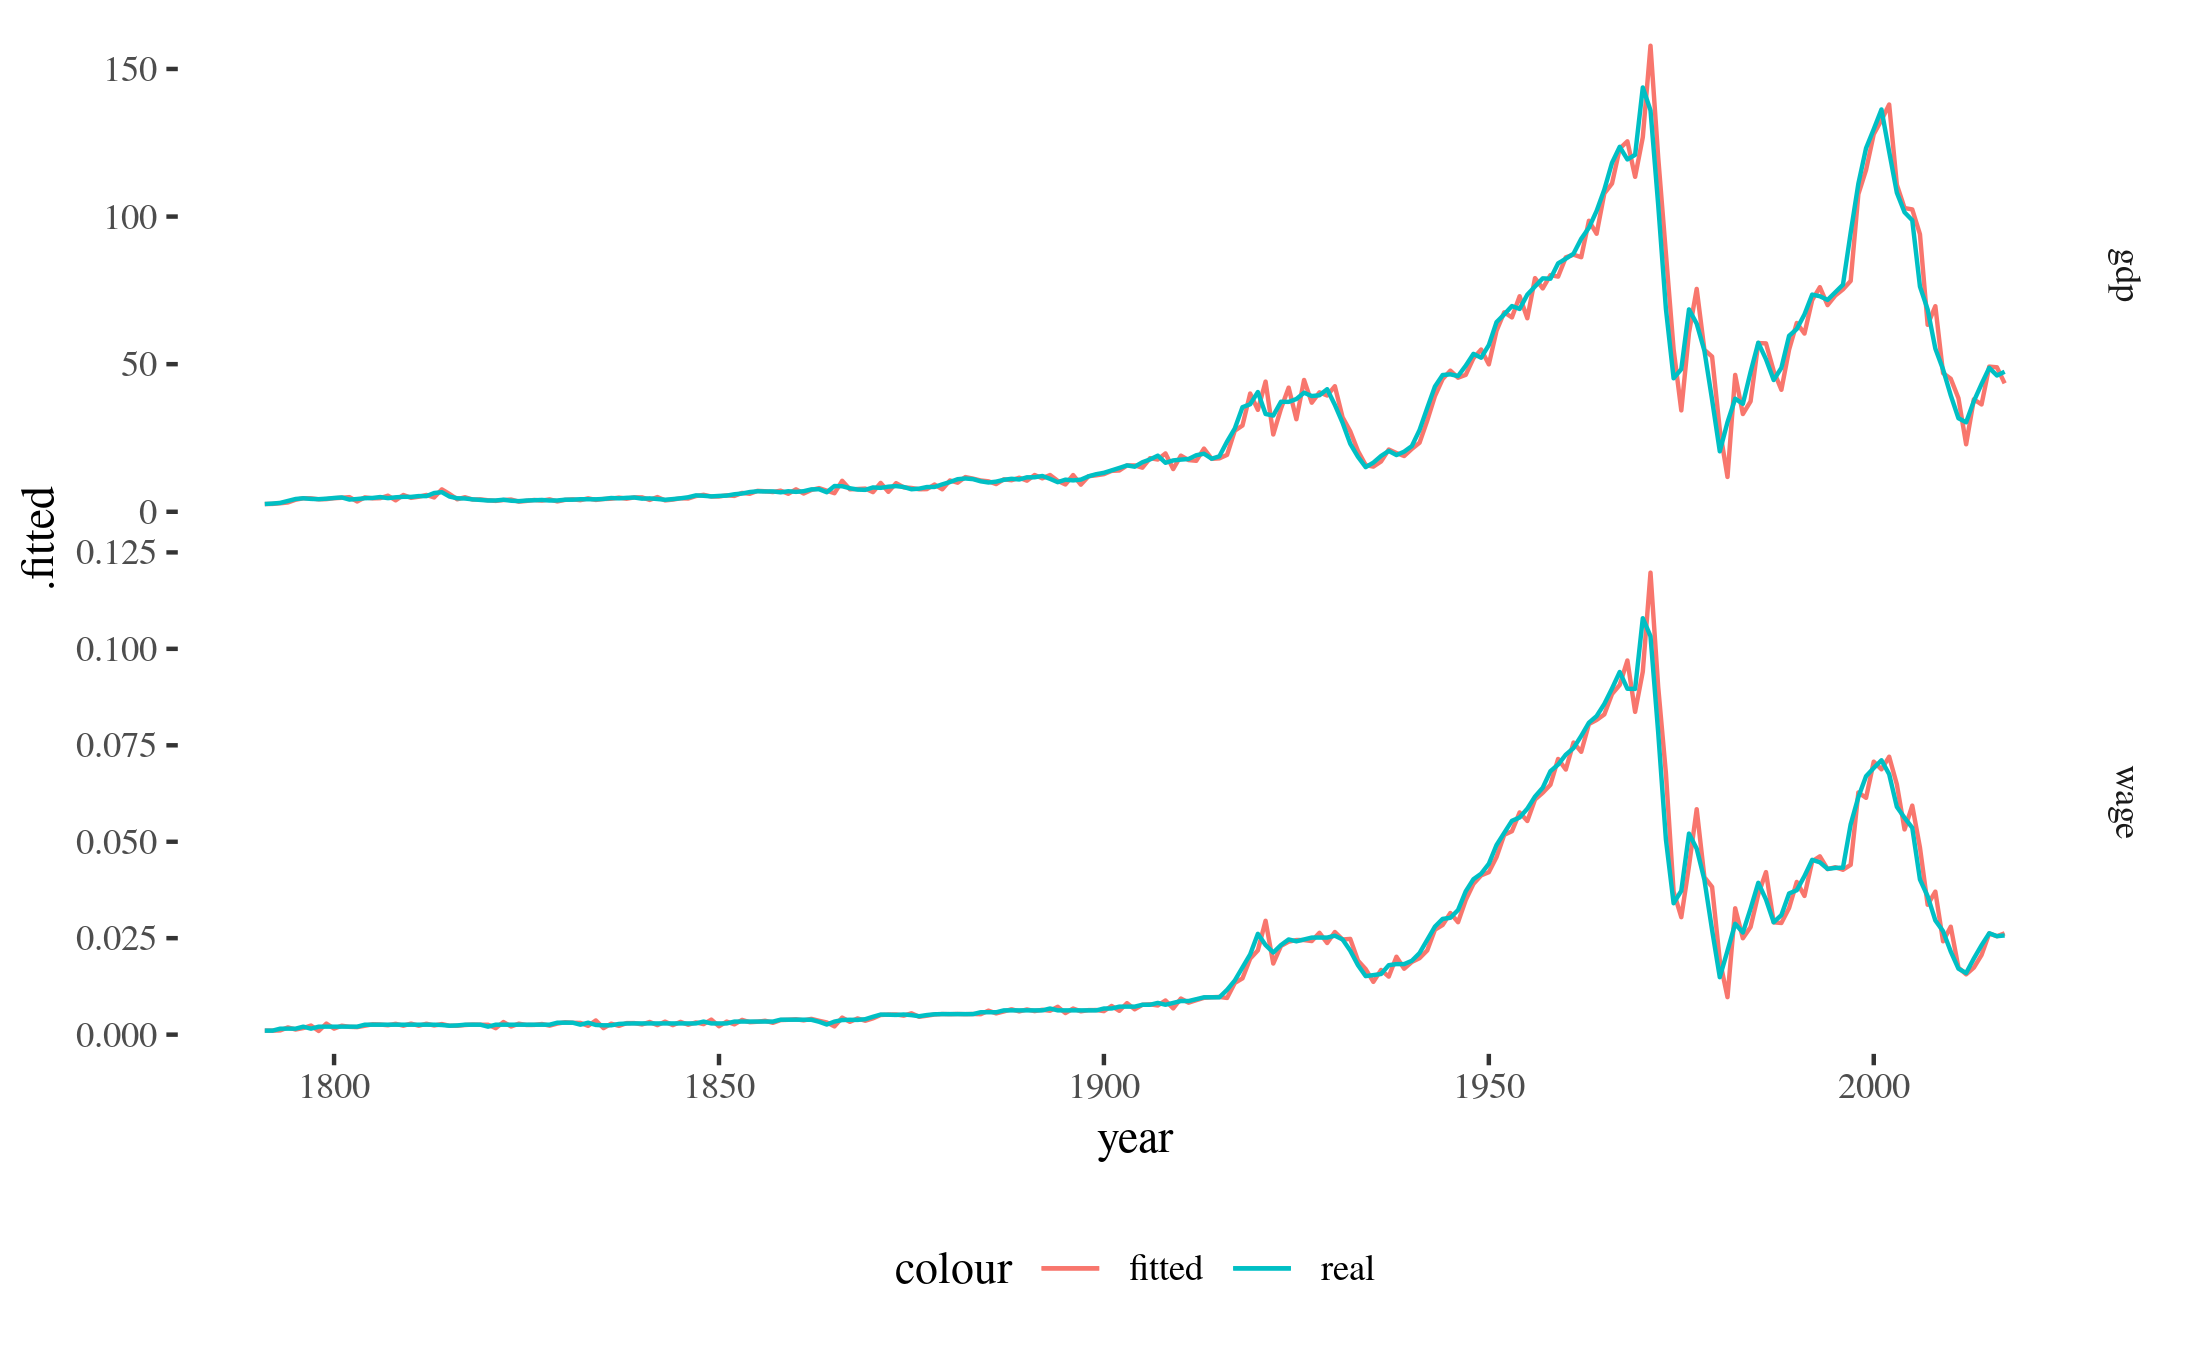
\includegraphics[width=0.8\linewidth]{arima_tot.png}
	\caption{Predicción ARIMA} \label{fig:arima}
\end{figure}

\section{Wavelets}

\begin{figure}[H]
	\centering
	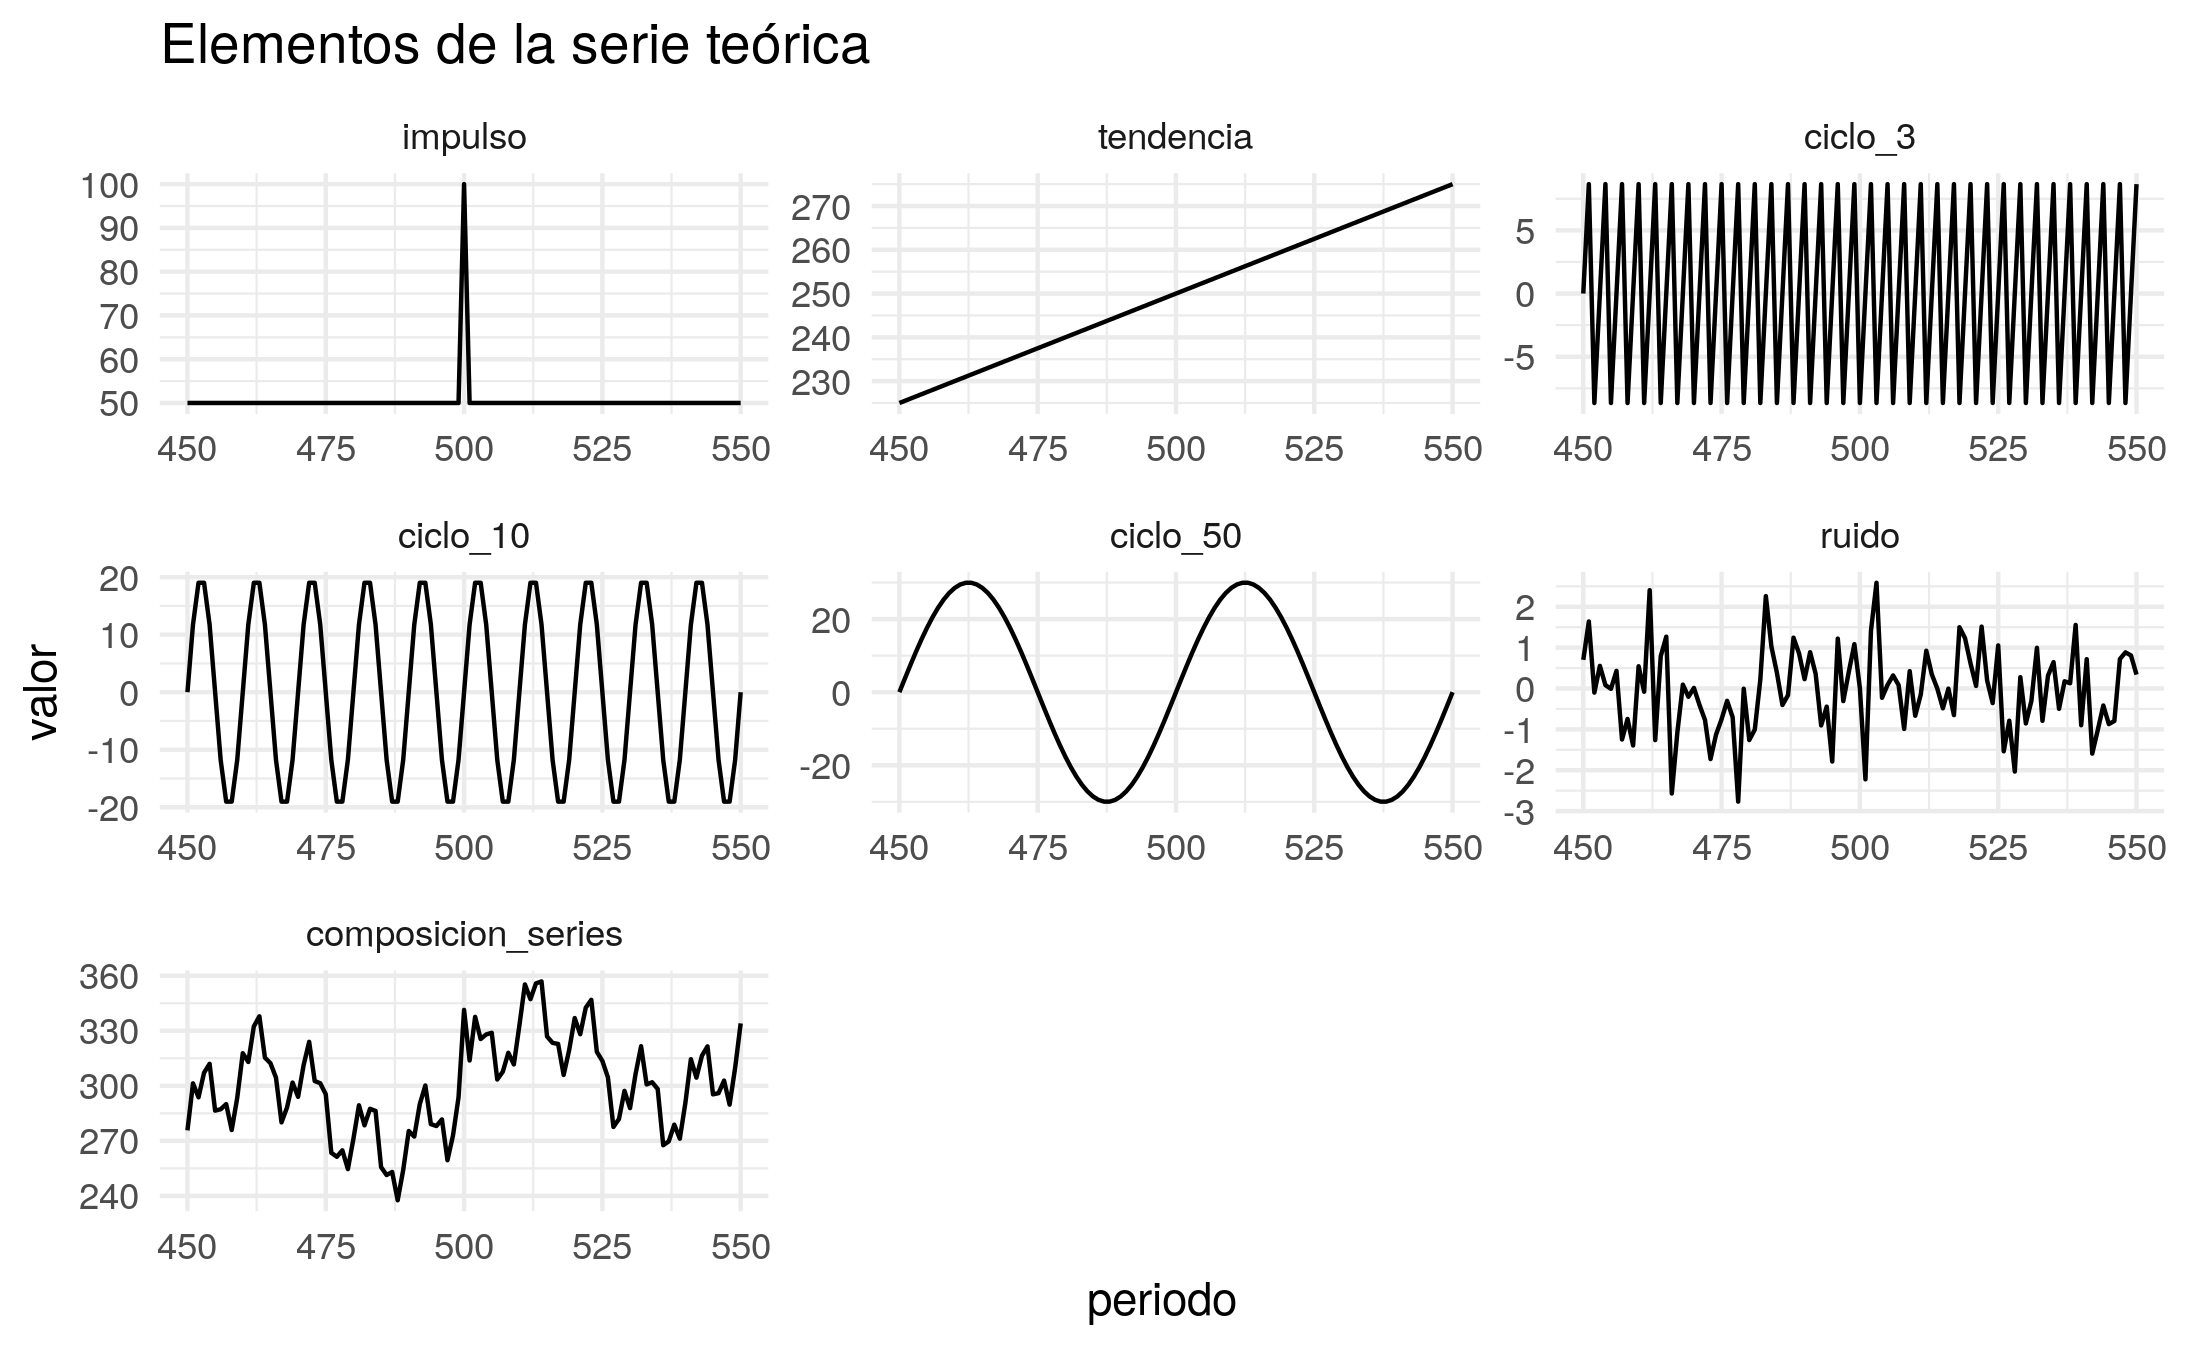
\includegraphics[width=\linewidth]{serie_teorica.PNG}
	\caption{Serie Teórica} \label{fig:serie_teorica}
\end{figure}


\begin{figure}[H]
	\centering
	\subfigure[impulso]{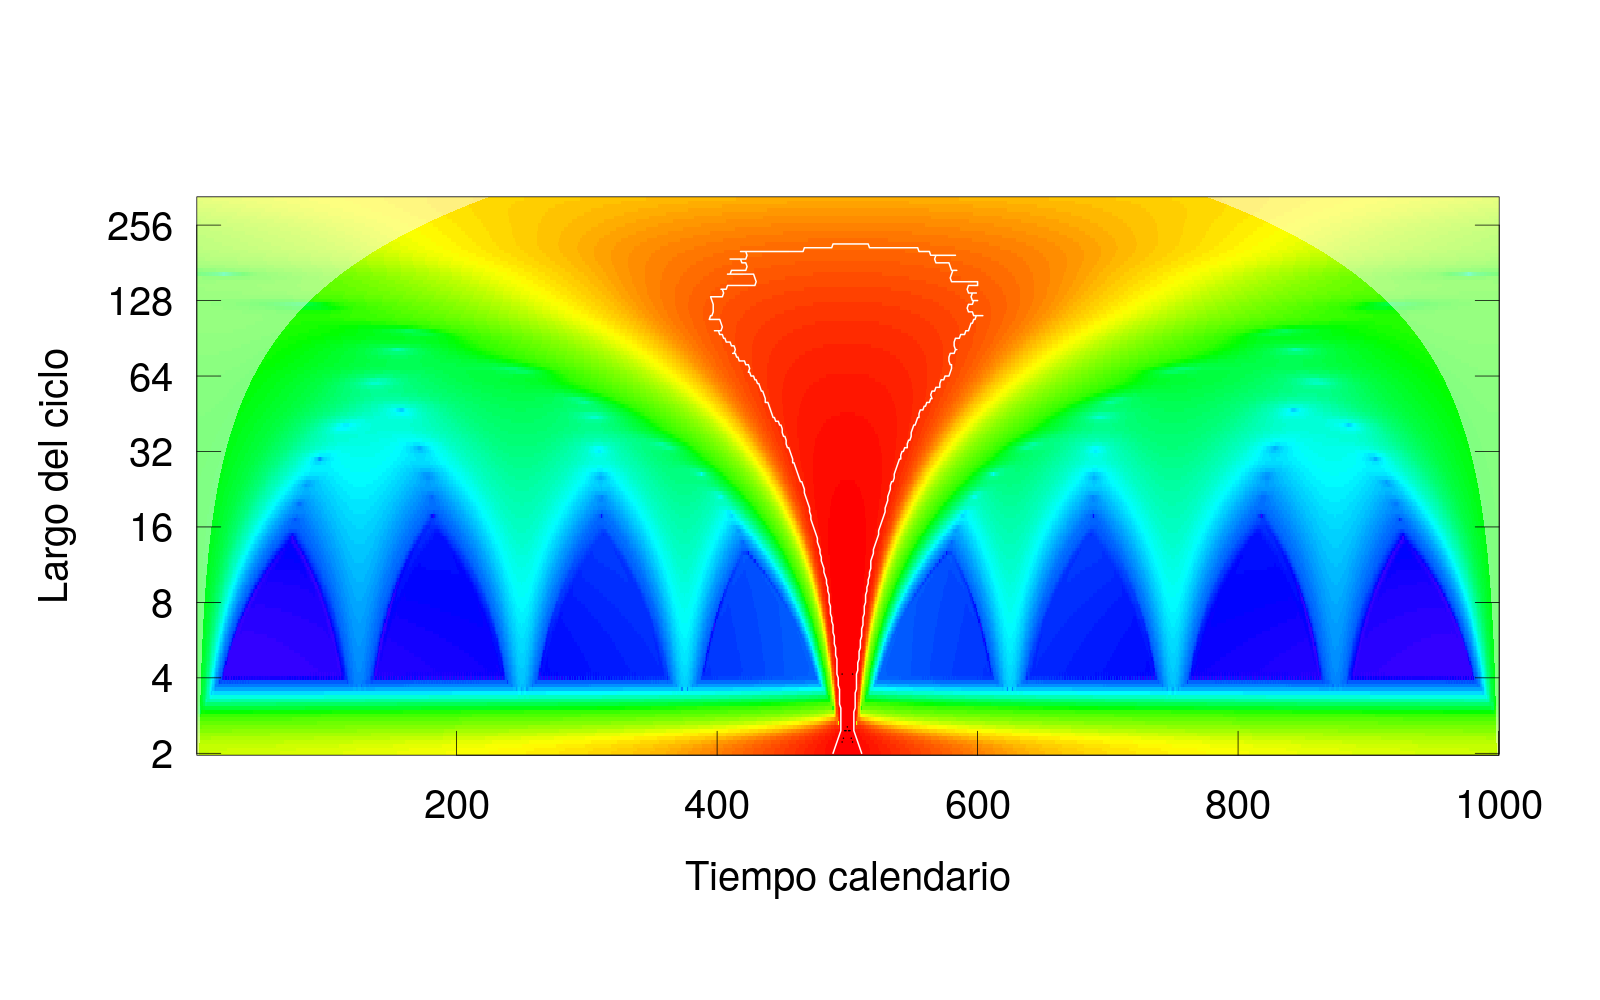
\includegraphics[width=0.49\linewidth]{espectograma_teorico_impulso.png}}
	\subfigure[tendencia]{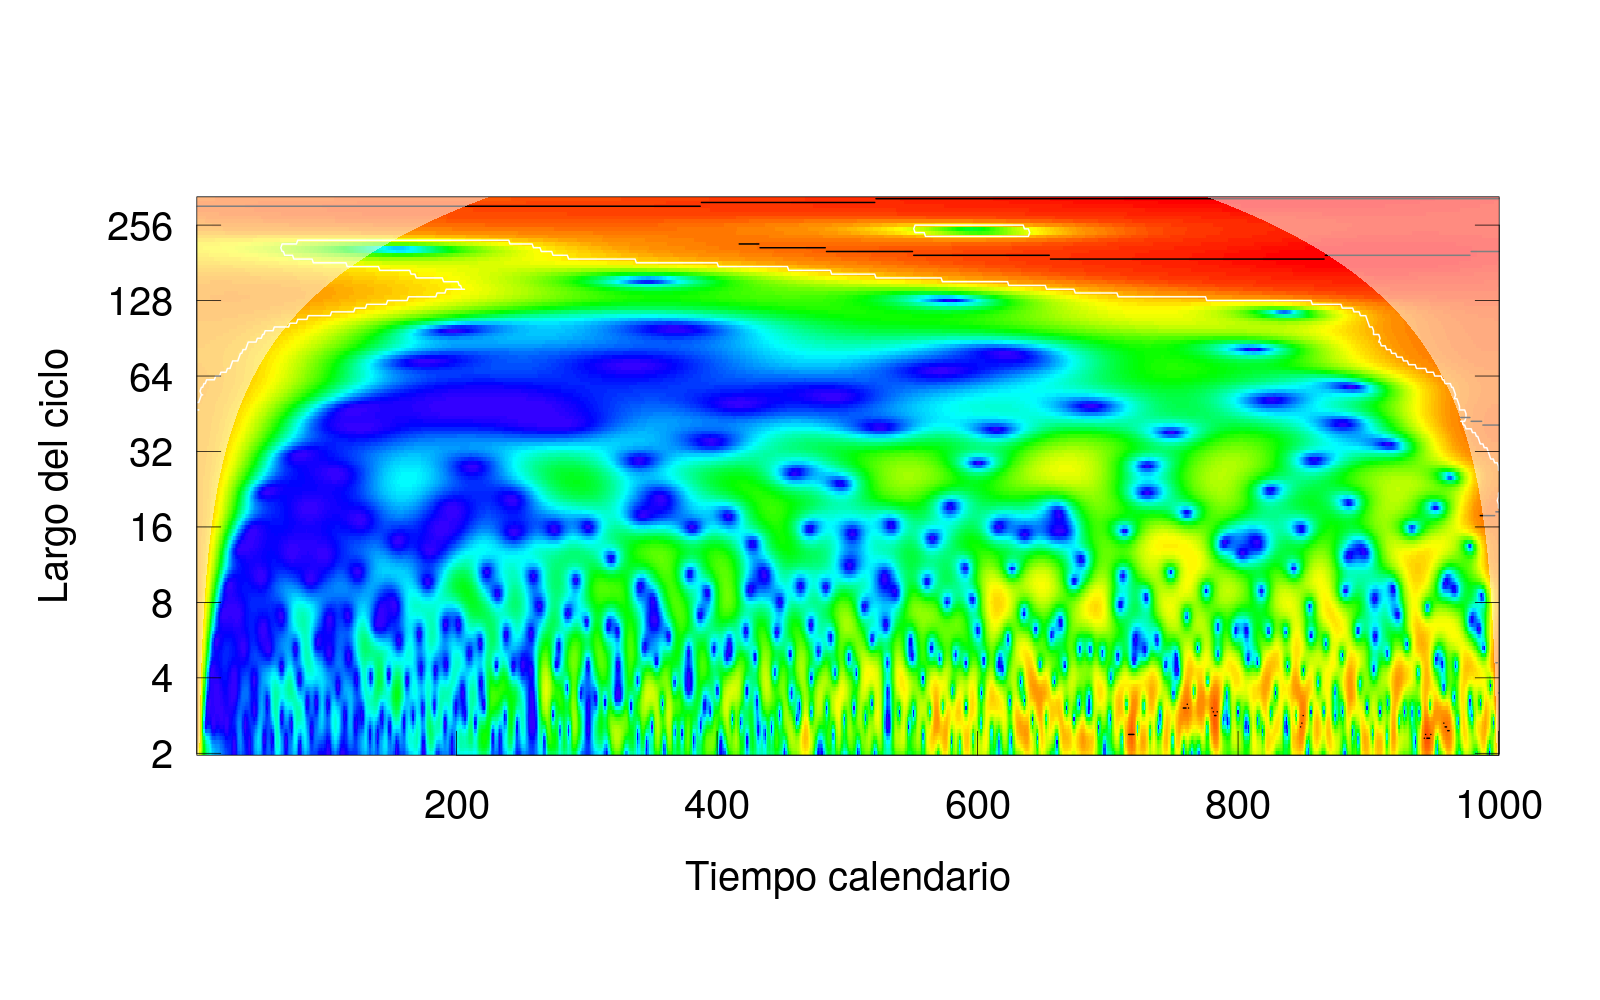
\includegraphics[width=0.49\linewidth]{espectograma_teorico_tendencia.png}}
	\subfigure[ciclo de 3 años]{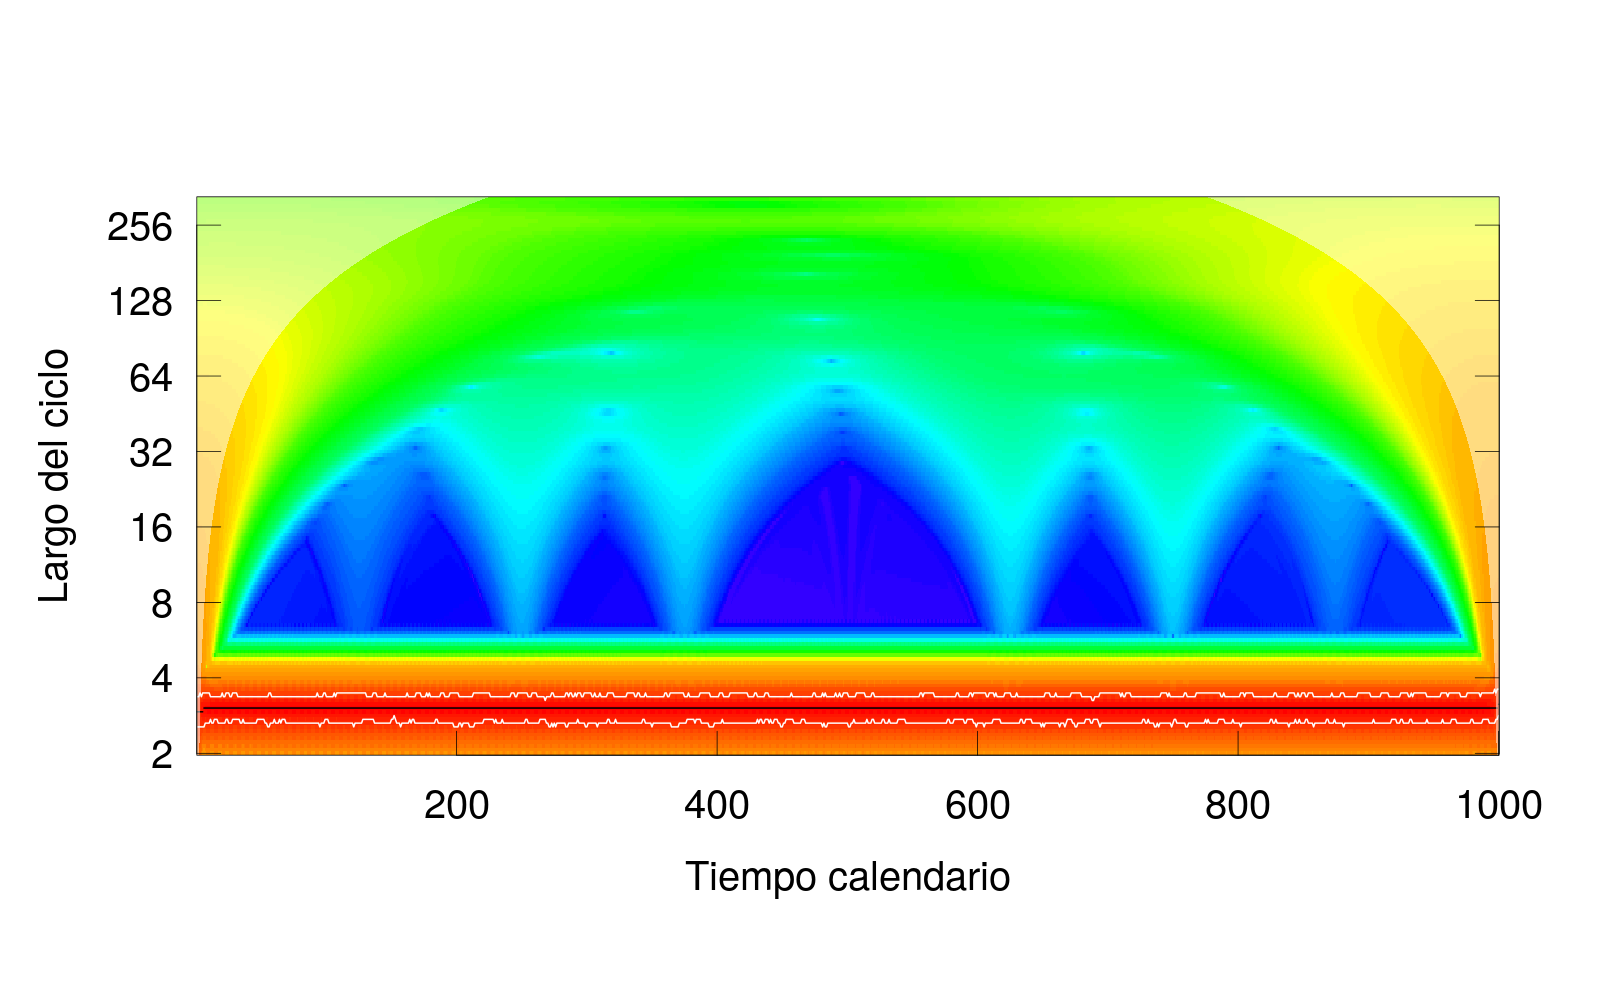
\includegraphics[width=0.49\linewidth]{espectograma_teorico_ciclo_3.png}}
	\subfigure[ciclo de 10 años]{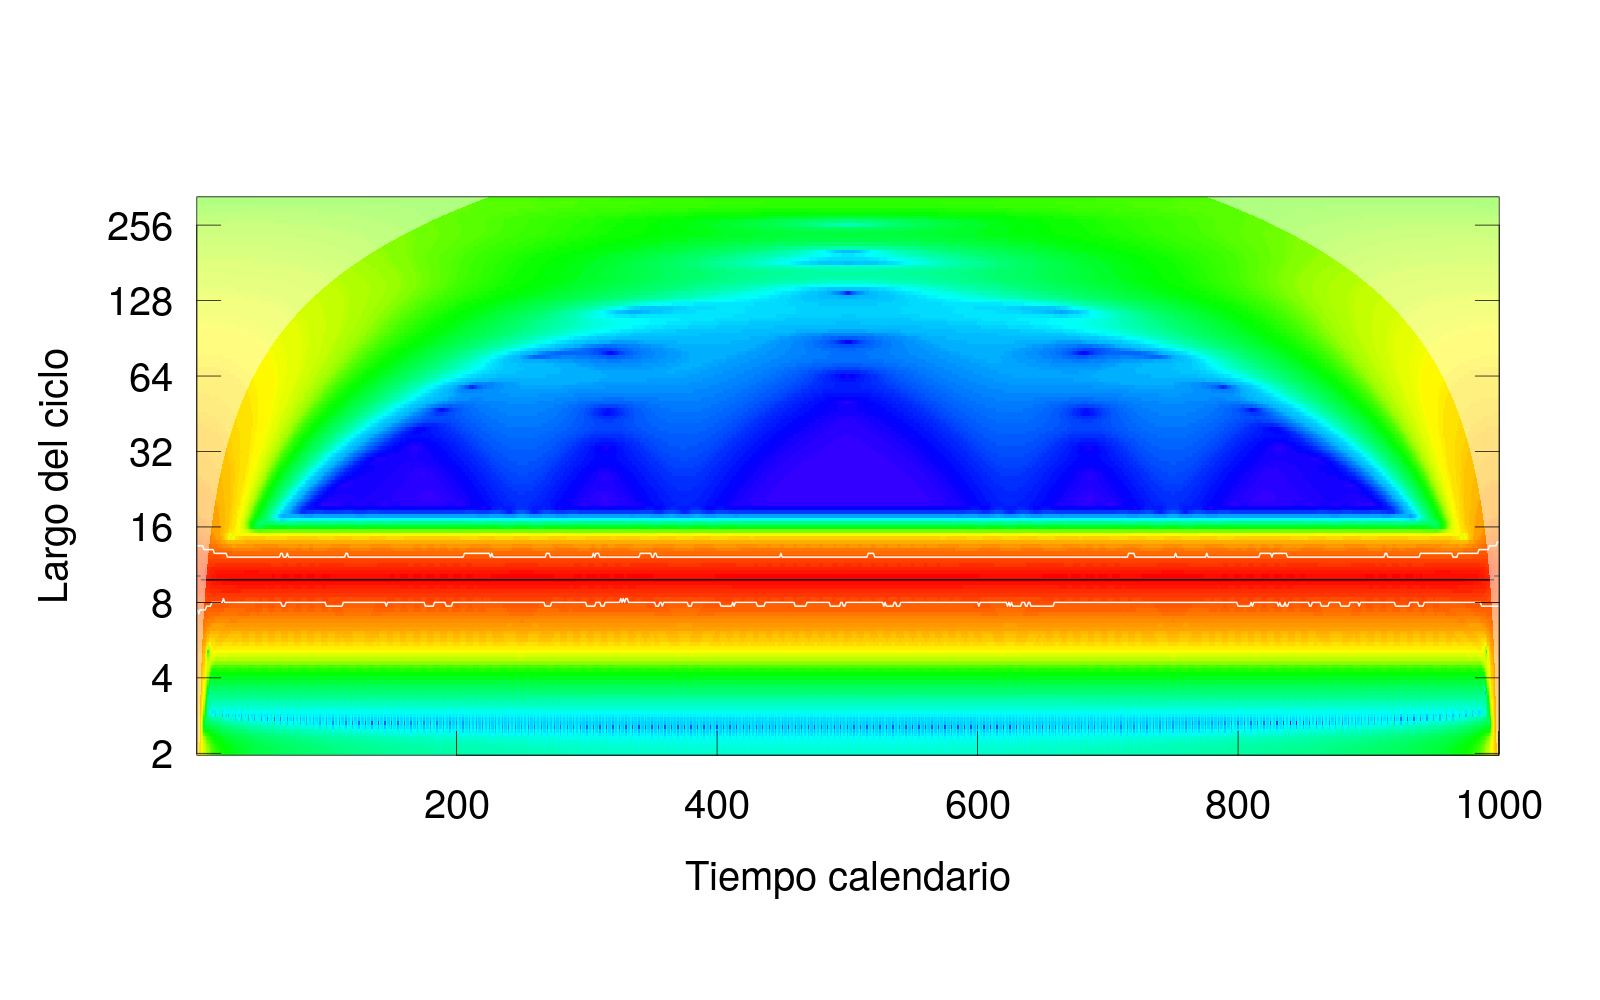
\includegraphics[width=0.49\linewidth]{espectograma_teorico_ciclo_10.png}}
	\subfigure[ciclo de 50 años]{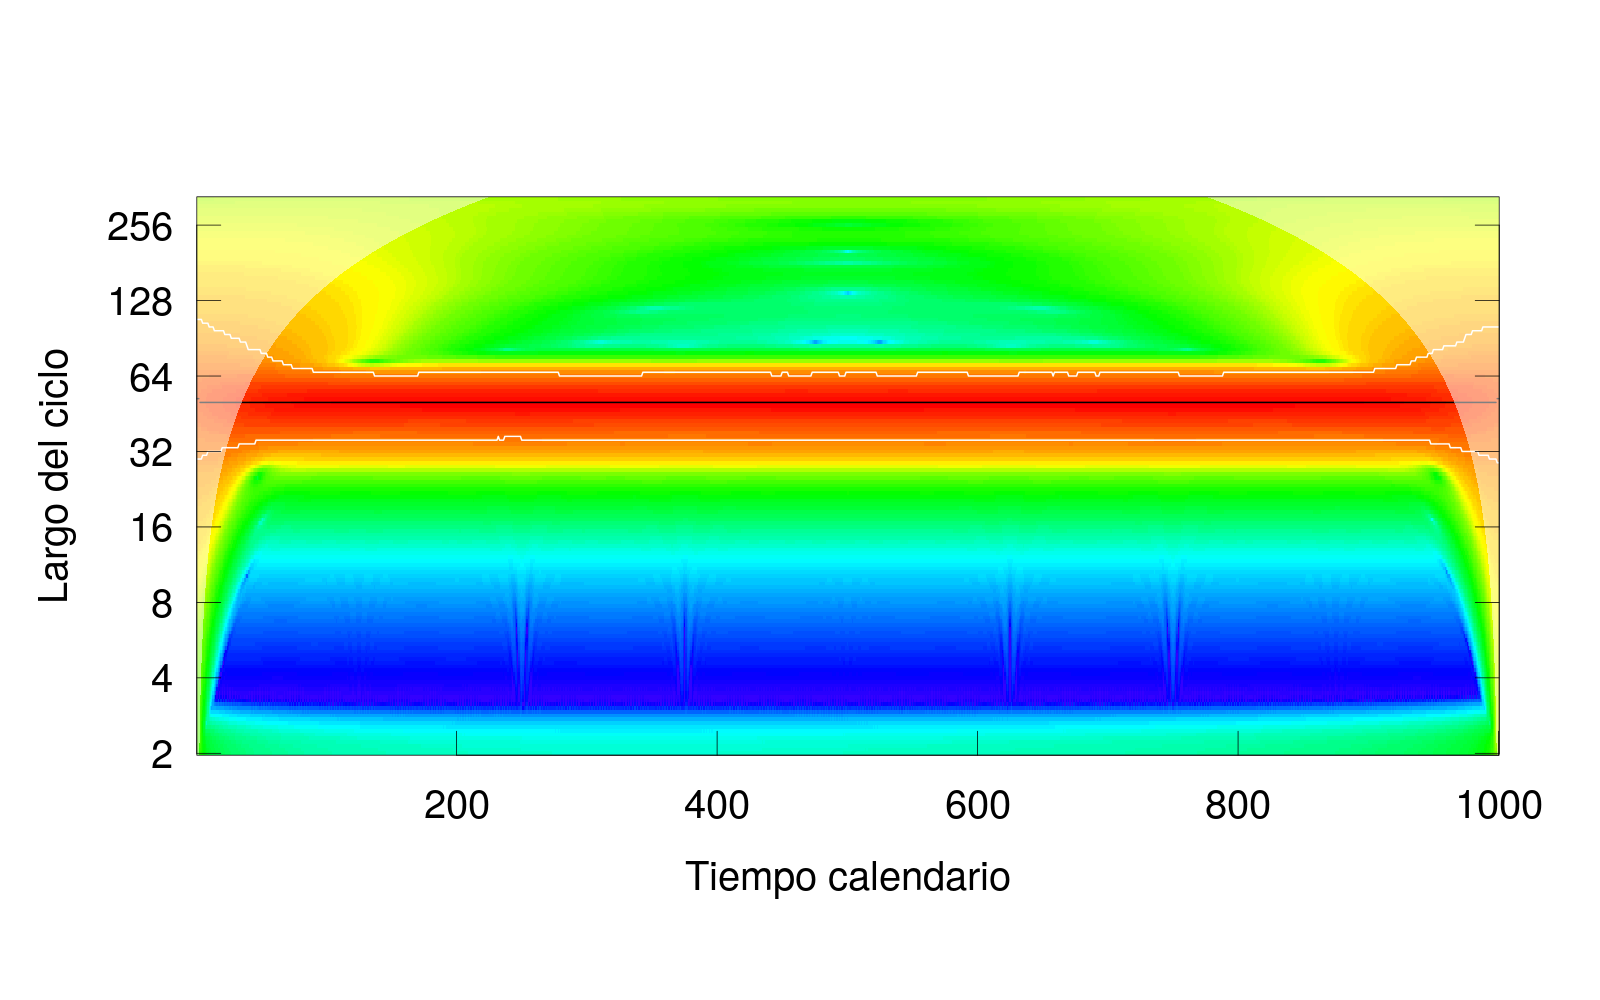
\includegraphics[width=0.49\linewidth]{espectograma_teorico_ciclo_50.png}}
	\subfigure[ruido normal]{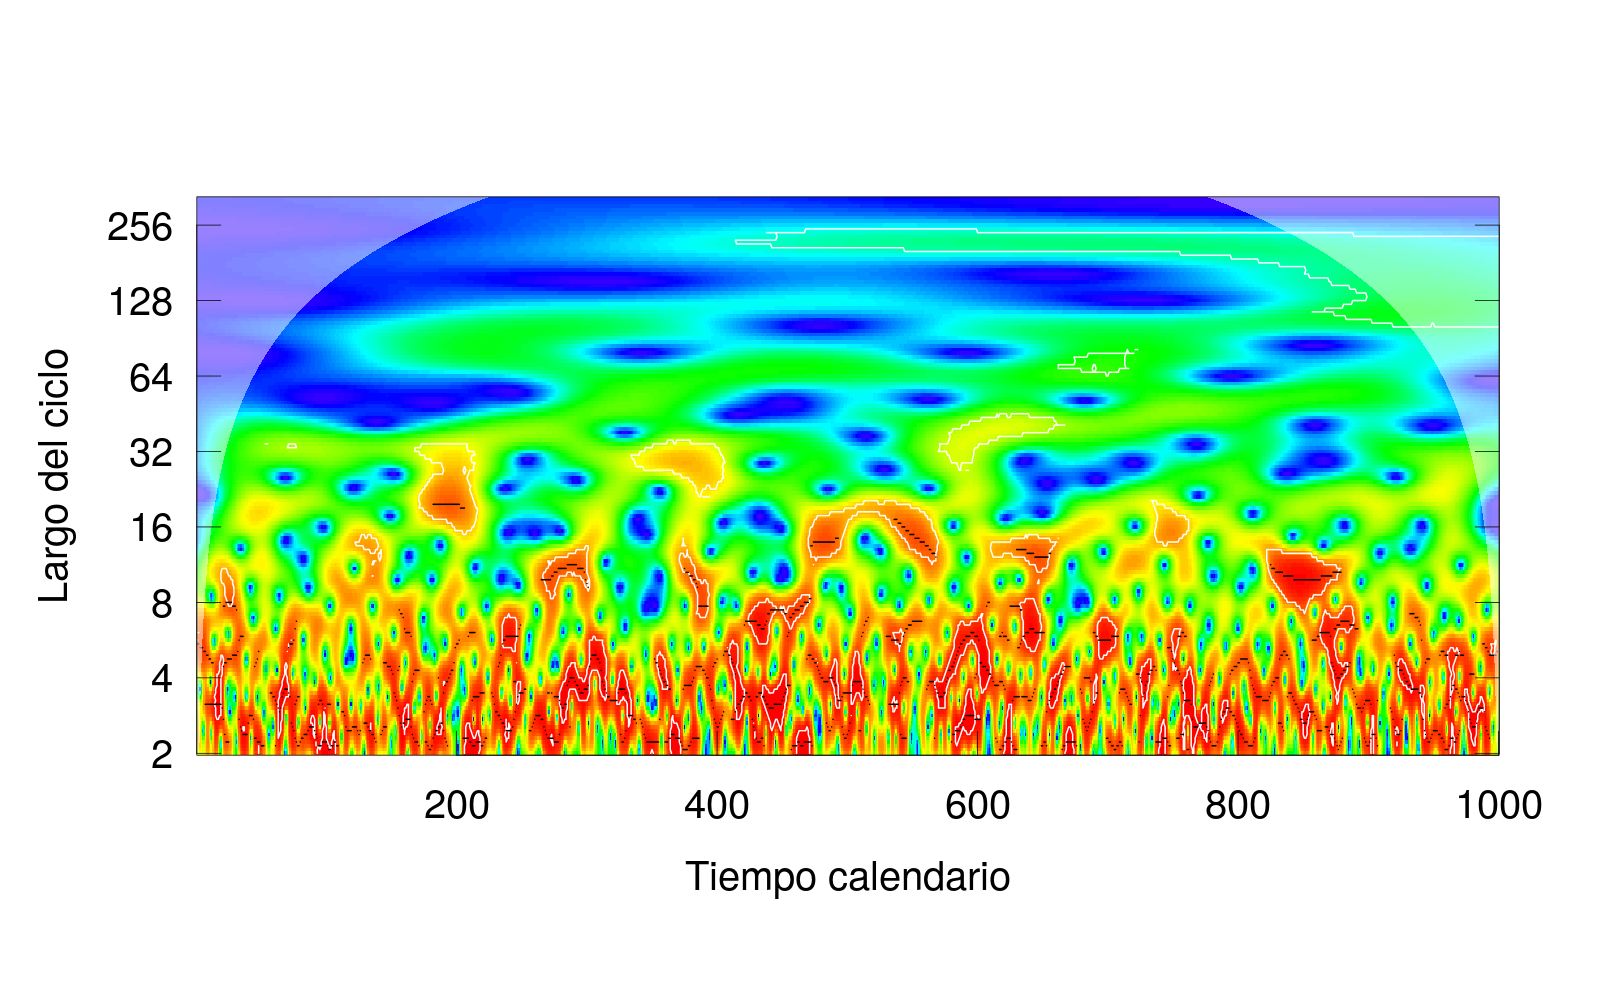
\includegraphics[width=0.49\linewidth]{espectograma_teorico_ruido.png}}
	\subfigure[composición de series]{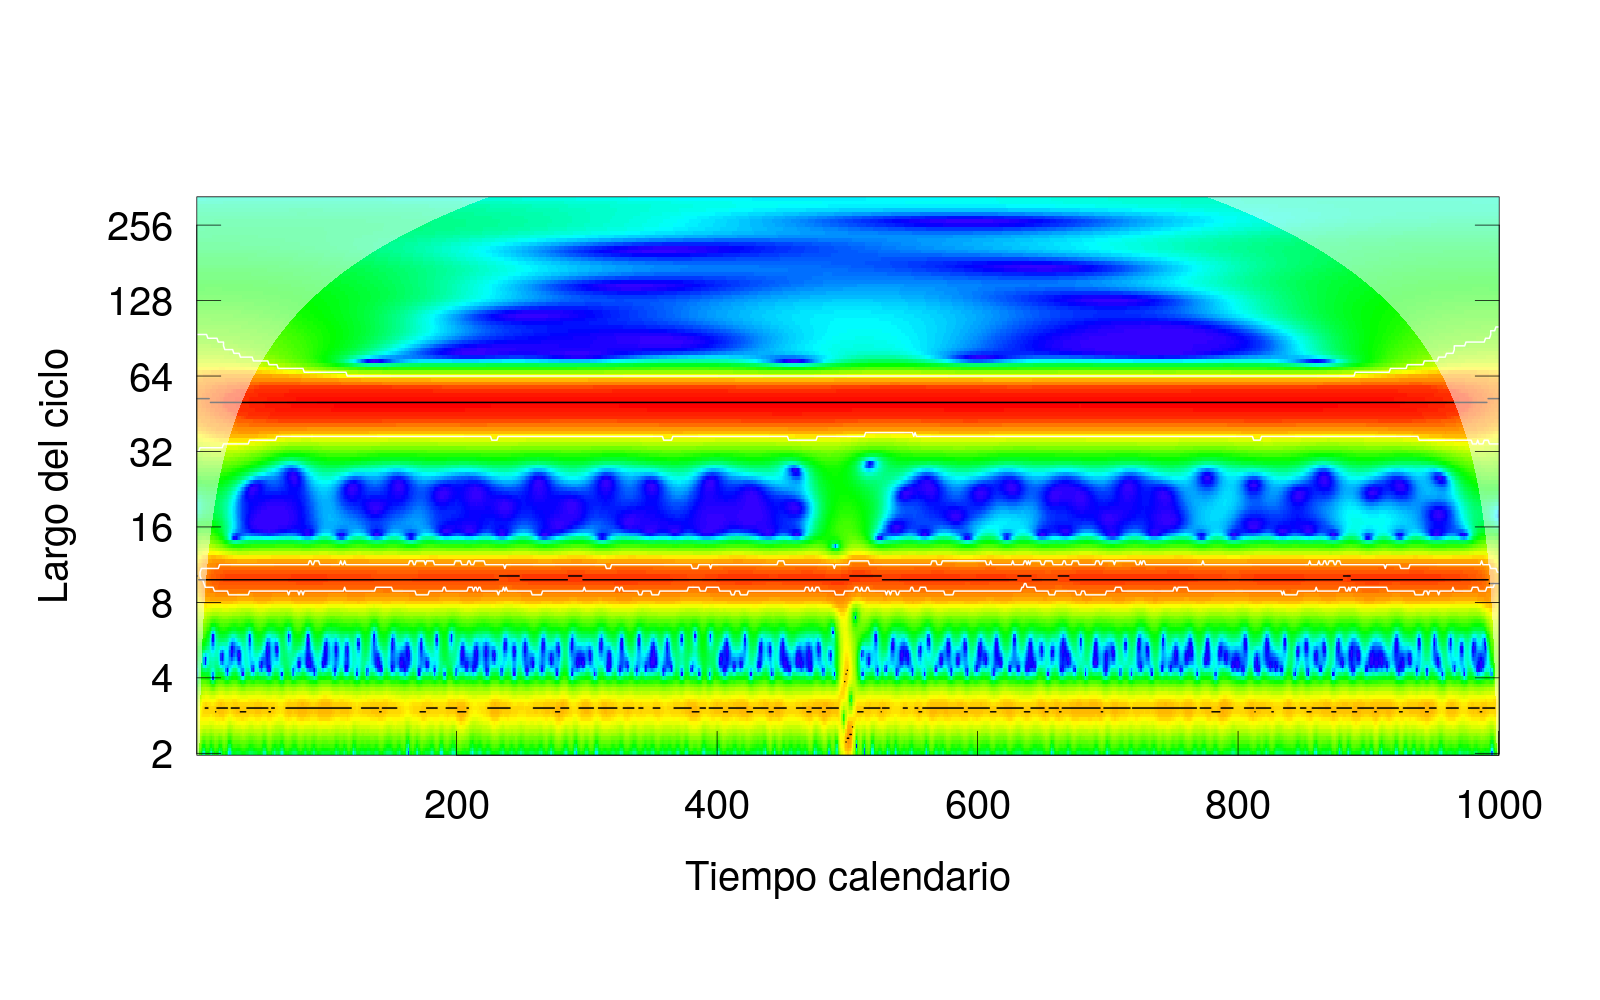
\includegraphics[width=0.75\linewidth]{espectograma_teorico_composicion_series.png}}
	\caption{Espectogramas Teóricos} \label{fig:espect_teo}
\end{figure}


\begin{figure}[H]
	\centering
	\subfigure[PBI]{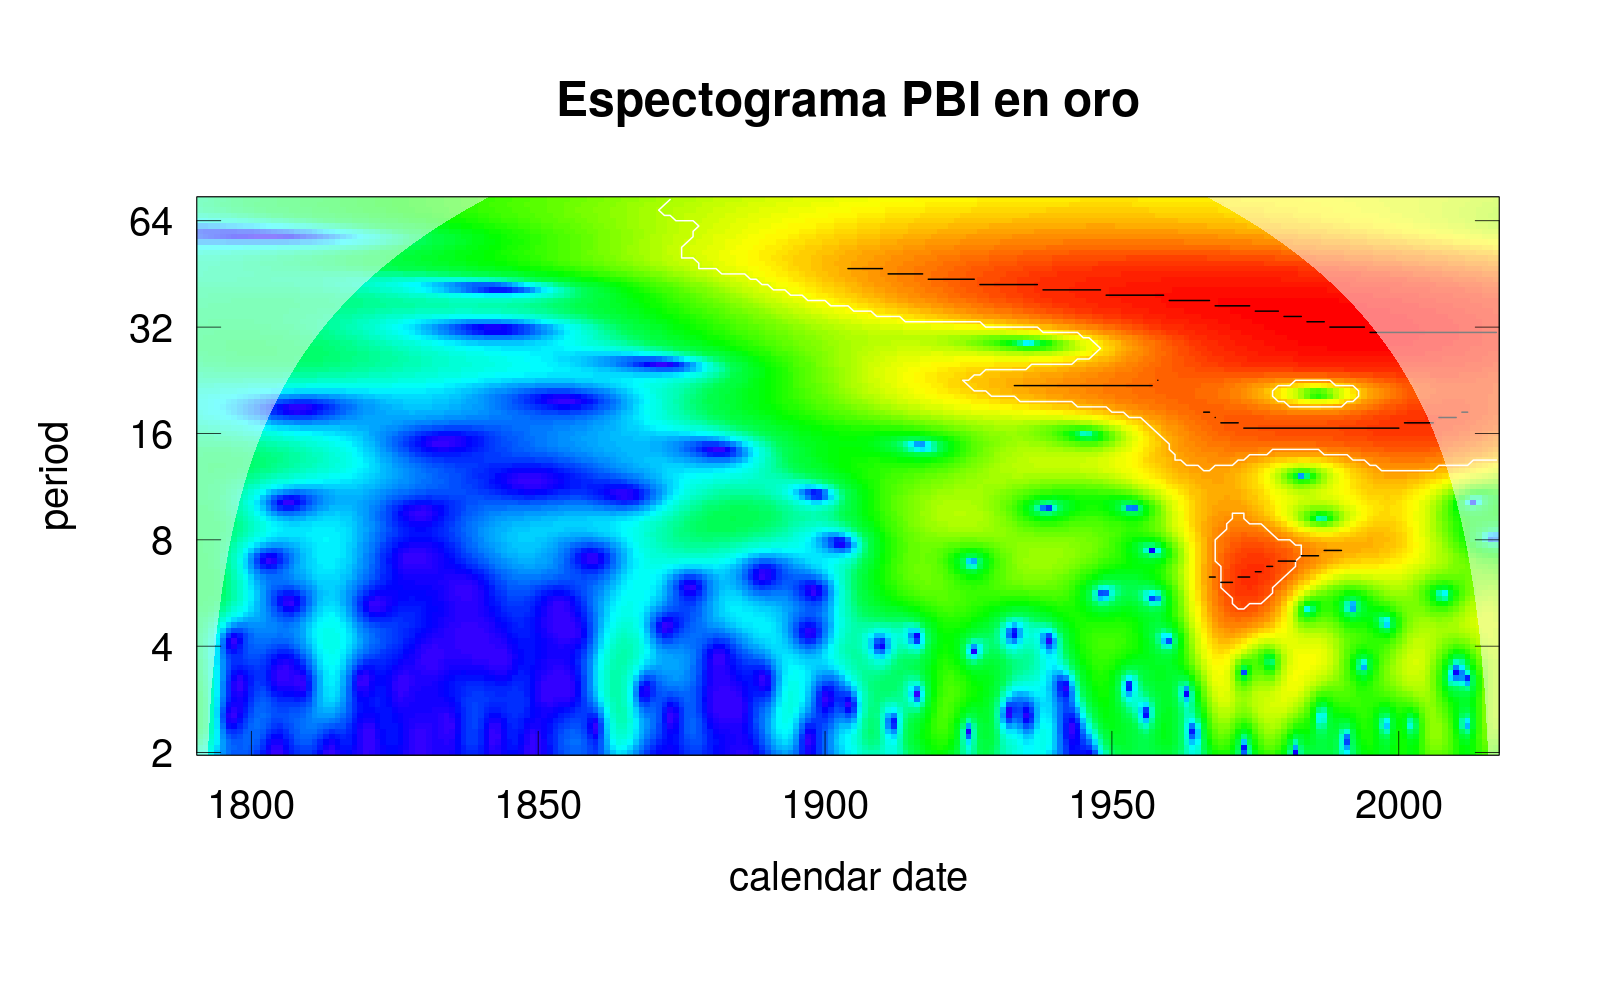
\includegraphics[width=0.75\linewidth]{espectograma_gdp.png}}
	\subfigure[$log(PBI)$]{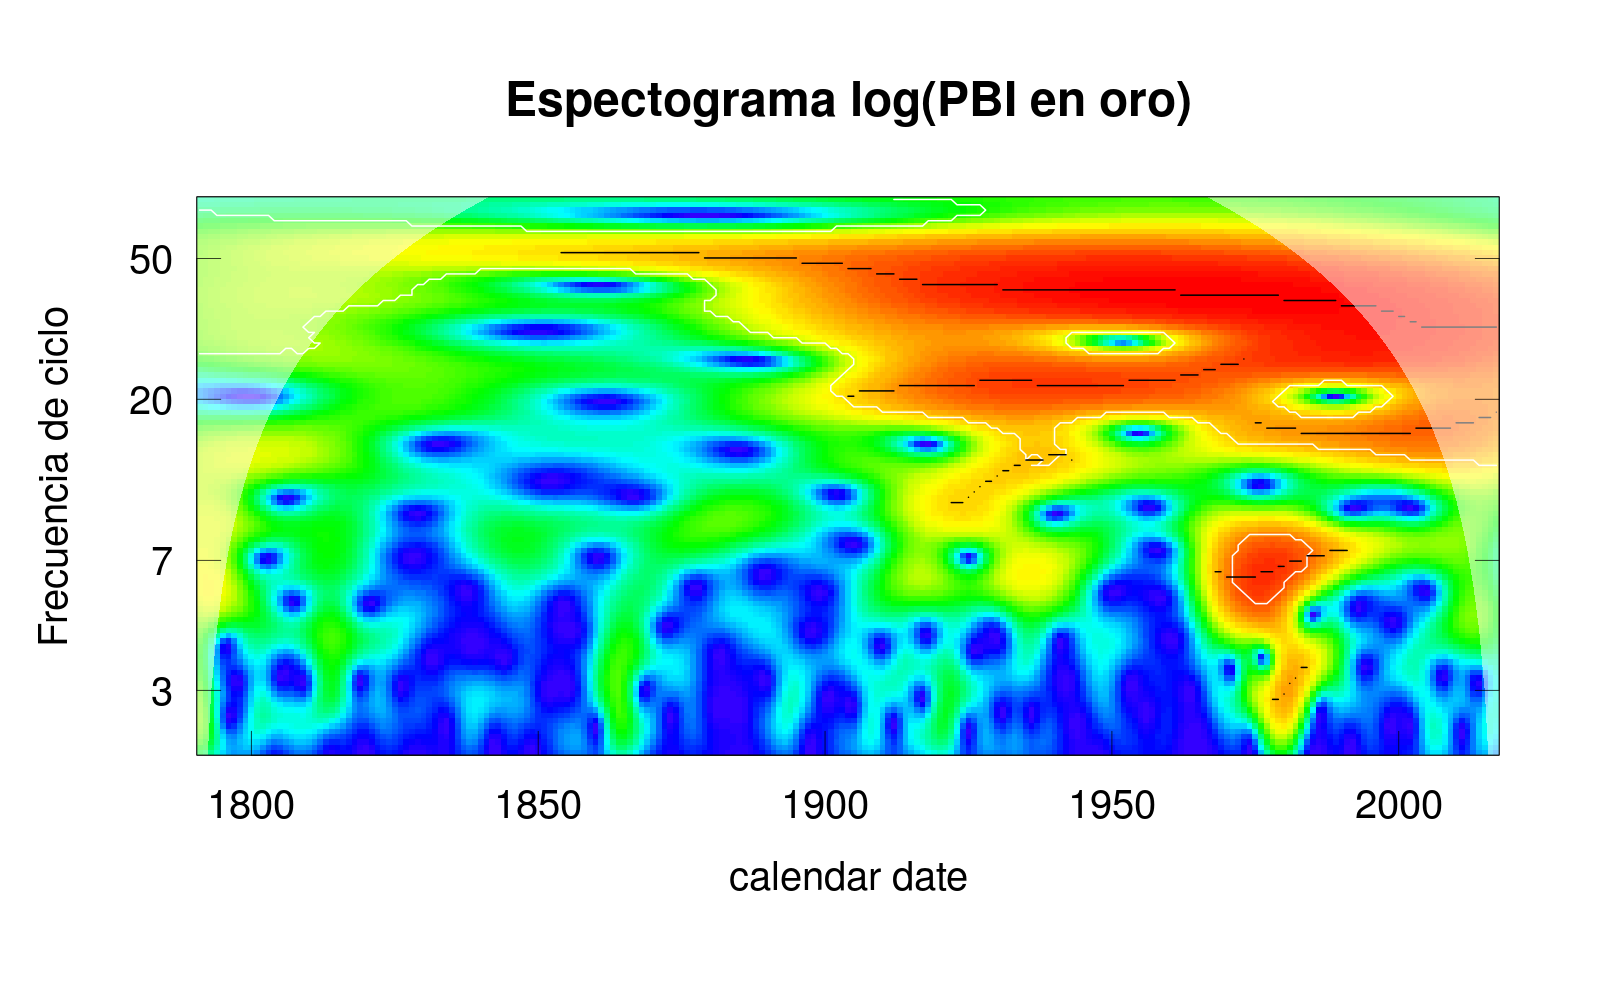
\includegraphics[width=0.75\linewidth]{espectograma_log_gdp.png}}
	\caption{Espectograma PBI en oro} \label{fig:espect_PBI}
\end{figure}

\begin{figure}[H]
	\centering
	\subfigure[Salario]{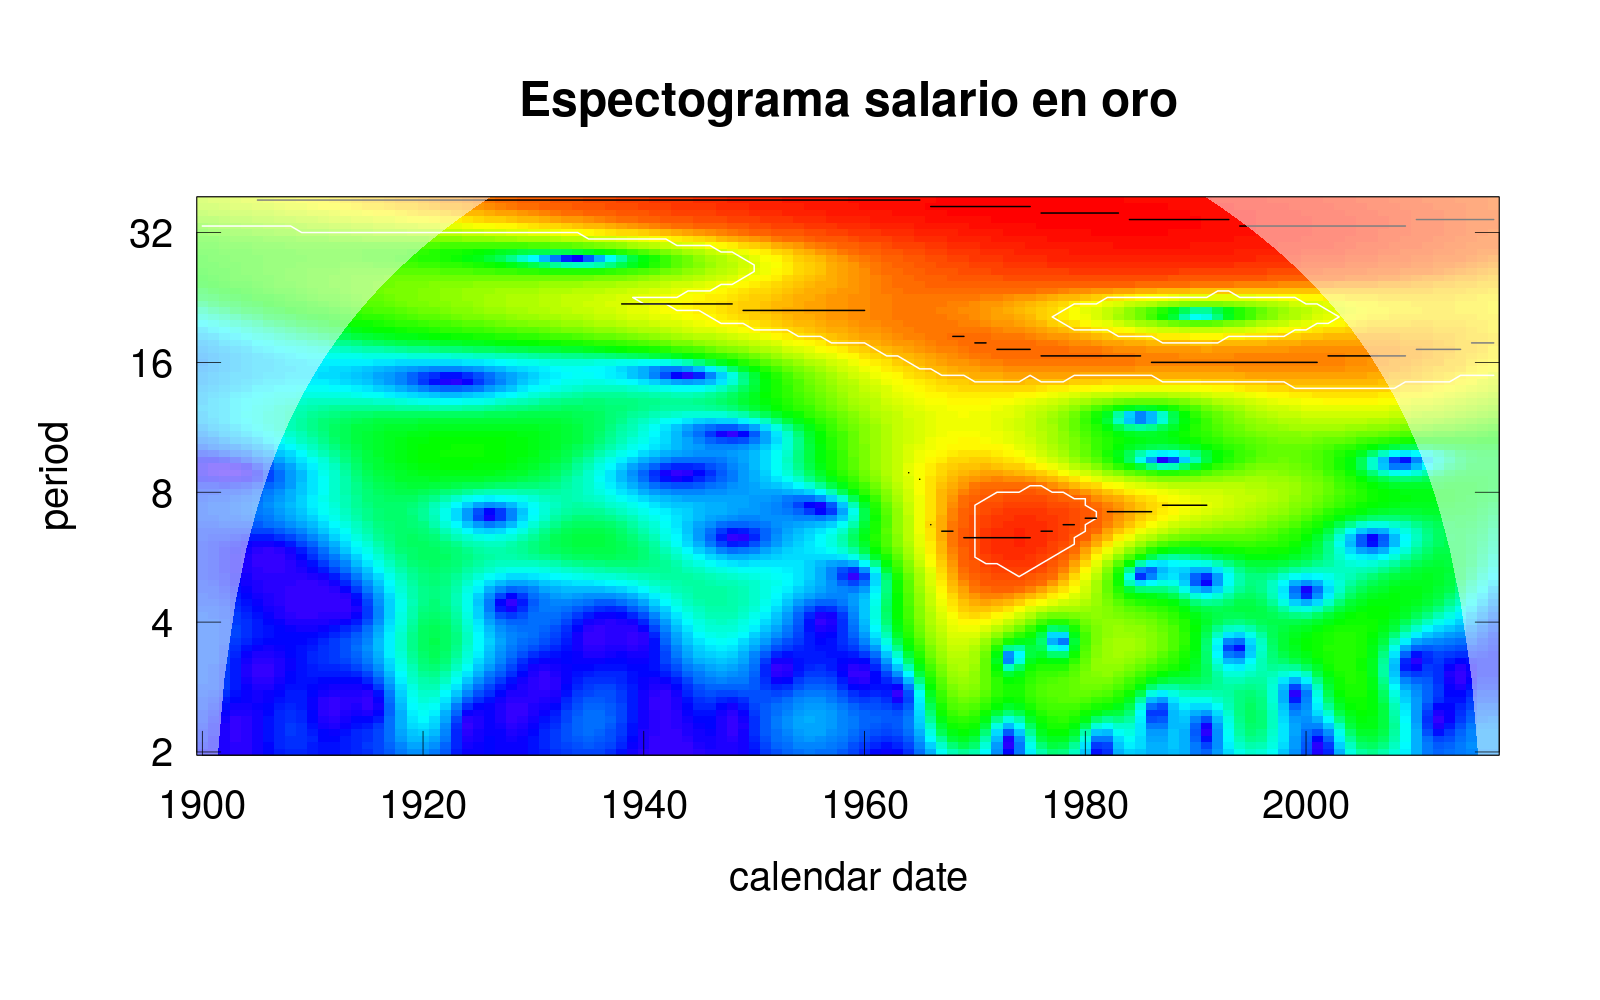
\includegraphics[width=0.75\linewidth]{espectograma_wg.png}}
	\subfigure[$log(Salario)$]{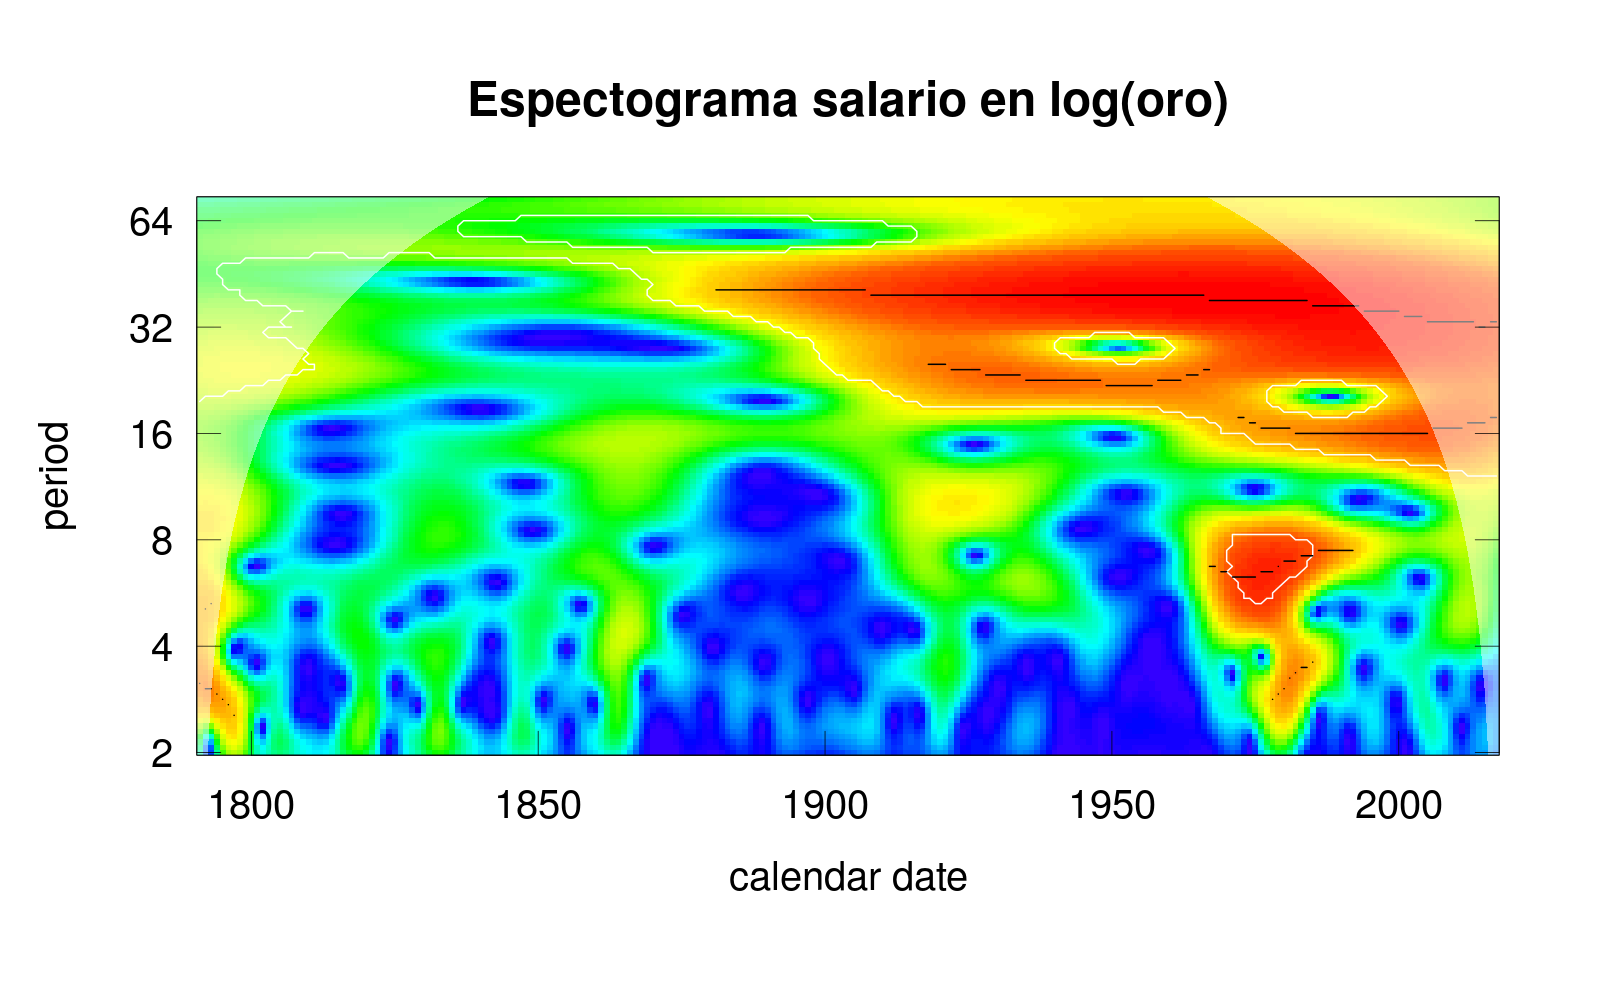
\includegraphics[width=0.75\linewidth]{espectograma_log_wg.png}}
	\caption{Espectograma Salario en oro} \label{fig:espect_wg}
\end{figure}



\section{Conclusiones}





\end{document}